\documentclass[]{interact}
\usepackage[T1]{fontenc}
\usepackage{lmodern}
\usepackage{graphicx}
\usepackage{booktabs,array}
\usepackage{amsmath,amssymb}
\usepackage{natbib}
\usepackage{url}
\usepackage[hidelinks]{hyperref}
\hypersetup{pdftitle={Causal residual calibration for traffic forecasting with delayed and lost sensor feedback},pdfauthor={Shishir Singh Chauhan}}
\bibpunct[, ]{(}{)}{;}{a}{}{,}
\renewcommand\bibfont{\fontsize{10}{12}\selectfont}
\newcounter{algorithm}
\newcommand{\ms}{\mathrm{m\,s^{-1}}}
\newcommand{\FAR}{\textsc{FAR-Cal}}
\begin{document}
\title{Causal residual calibration for traffic forecasting with delayed and lost sensor feedback}
\author{\name{Shishir Singh Chauhan\thanks{CONTACT Shishir Singh Chauhan. Email: shishir.chauhan@jaipur.manipal.edu}}
\affil{Manipal University Jaipur, off Ajmer--Jaipur Expressway, Dahmi Kalan, Rajasthan 303007, India}}
\maketitle
\noindent Approximate manuscript prose word count: 8926 (excluding references, tables, captions and displayed equations).\par

\begin{abstract}
Traffic forecasting intervals depend on both observed inputs and feedback about realised outcomes. Sensor reporting failures can interrupt these channels differently, leaving online calibration without current residual evidence. We develop a causal replay benchmark and an asymmetric residual calibration method that combines spatial pooling, context matching, target-age weighting and historical fallback. Evaluation uses METR-LA, PEMS-BAY and controlled SUMO datasets with frozen forecasting backbones, independent controls and registered reporting stress. The method satisfies a joint interval-score and coverage rule in twelve of sixteen real-data backbone cells. Fresh simulation validation succeeds with delayed feedback, whereas permanent-loss transfer misses the coverage floor. Seven full component ablations identify thirteen adverse removals, four beneficial removals and twenty-five inconclusive effects. Results support conditional gains rather than universal superiority. Explicit independently configured release schedules, immutable forecasts and publicly accessible evidence make the comparisons independently reproducible, without asserting identifiable correction of selectively missing outcomes or operational traffic-control benefits.
\end{abstract}
\begin{keywords}
Traffic forecasting; prediction intervals; sensor outages; delayed feedback; uncertainty calibration; reproducibility
\end{keywords}

\section{Introduction}\label{sec:introduction}
Traffic forecasting is increasingly framed as a prediction problem on a network, but an uncertainty service also depends on a reporting process. A speed measurement has a physical timestamp, a delivery timestamp and a role in subsequent decisions. If a detector gateway stops reporting, the forecasting model loses recent inputs. The calibration module also loses the realised outcomes needed to assess forecasts already issued. Treating these two losses as interchangeable hides an important distinction: a predictor may continue producing plausible values while the residual evidence supporting its intervals becomes stale. The uncertainty problem therefore concerns information availability as well as traffic dynamics.

The practical motivation is straightforward. An operator receiving a forecast needs to know how much confidence to place in it during degraded sensing. A narrow interval based on a healthy historical period can be misleading after a correlated outage, even when its point forecast changes little. Conversely, widening every interval indiscriminately can make the service uninformative. A useful evaluation must consider coverage together with interval width and the penalty for missed outcomes. It must also retain difficult targets in the scoring population when their reports are unavailable to calibration. Otherwise, removing the very outcomes most affected by failure can artificially improve reported performance.

Delayed feedback presents a second difficulty. A backlog released after restoration may contain many residuals, yet describe conditions several hours earlier. Delivery recency is then a poor proxy for relevance. Permanent loss creates a different information deficit because the missing residuals never enter the live archive. A method that succeeds with delayed packets need not succeed when outcomes disappear. These mechanisms motivate retaining target timestamps, issuing immutable intervals and distinguishing input release from feedback release. The proposed replay follows this ordering explicitly rather than giving the calibrator access to evaluator truth or retrospectively revising uncertainty after the outcome becomes known.

Spatial information offers a possible response, but creates its own risks. Nearby sensors can supply residual evidence when a local detector is silent. Their errors can also be correlated, and their speed regimes need not match the affected location. Context matching and temporal weighting may improve relevance while reducing effective support. An historical archive can stabilise sparse updates, but can preserve obsolete residual behaviour. The methodological question is consequently not whether every available record should be pooled. It is how the usefulness of live, neighbouring and historical evidence changes under a specified reporting process, and how those choices affect interval quality on held-out data.

Traffic predictors provide several ways to represent network dependence. Graph WaveNet and DCRNN use graph-based temporal modelling, whereas STID and STAEformer use identity information and adaptive embeddings \citep{wu2019,li2018,shao2022,liu2023}. The present study does not seek to replace these forecasting architectures. It holds each fitted predictor fixed and compares calibrators on identical forecasts, scales and evaluation masks. This separation makes a paired score difference interpretable as a calibration effect conditional on the backbone. Repeating the comparison across backbones then tests transfer without confusing a stronger point predictor with a better use of outcome feedback.

Conformal and adaptive inference offer relevant foundations, but their assumptions must be respected. ACI adjusts uncertainty from sequential coverage errors, and multistep extensions account for the ordinary wait until a forecast target occurs \citep{gibbs2021,hallberg2024}. Recent work also studies delayed or corrupted feedback directly \citep{elhalabi2026,wang2026}. Accordingly, feedback-aware uncertainty is not claimed as an unexplored general topic. Our narrower focus is a traffic replay with independently impaired input and outcome channels, correlated outages, permanent loss and auditable historical fallback. The proposed weighted signed-residual method is evaluated empirically; source theorems are not transferred to its modified reporting protocol.

The research has three connected objectives. First, it establishes an information boundary that prevents unavailable outcomes from entering calibration while allowing originally valid targets to remain assessable by the evaluator. Second, it evaluates whether asymmetric residual pooling improves the registered interval-score endpoint without falling below a prespecified coverage floor. Third, it investigates whether the result survives changes in network, forecasting backbone, reporting severity and individual components. Each objective requires a different comparison. Fresh simulation episodes assess the locked candidate; matched-rate controls examine an alternative outage geometry; component removals assess mechanisms while retaining the same point and scale caches.

The empirical design combines METR-LA, PEMS-BAY and controlled SUMO simulations. Real-data inference uses chronological partitions and fault-focused hourly origins, while simulation permits full episode evaluation under separately specified physical and reporting events. The study includes core conditions, independent controls, one-factor stress and seven complete component ablations. The breadth is useful only if scope differences remain visible. An hourly network audit is not a complete five-minute deployment trial, and controlled simulation is not proof of field effectiveness. The manuscript therefore reports sampling rules, adaptation choices, uncertainty intervals and adverse findings alongside favourable results, rather than presenting a single aggregated ranking.

The main contribution is an executable causal benchmark coupled with a feedback-aware calibration design and a transparent account of its conditional performance. The final asymmetric method passes twelve of sixteen real-data backbone cells, but this aggregate conceals important differences between networks. Full ablations also reveal components whose removal improves score. Such findings constrain both mechanism claims and practical recommendations. No universal superiority, arbitrary-missingness coverage guarantee or identifiable correction for missing-not-at-random outcomes is asserted. Potential societal benefits motivate the work, while actual impacts on traffic control, safety, travel time or equity remain outside the demonstrated outcomes.

A reproducible comparison also needs recoverable provenance. Saved schedules, forecast identifiers, configuration hashes and originally valid masks allow readers to distinguish a statistical result from an interrupted runner or a reporting artifact. This accountability is also particularly important when evaluations are resumed, because existing verified stages remain evidence rather than being silently replaced.

The remainder of the paper follows the dependency order of the study. Section~\ref{sec:related} positions forecasting, missing-data reconstruction and sequential calibration. Section~\ref{sec:data} describes datasets and partitions. Section~\ref{sec:architecture} explains the information flow. Section~\ref{sec:math} formalises the model, and Section~\ref{sec:algorithm} details its algorithm. Section~\ref{sec:protocol} defines comparisons and inference. Section~\ref{sec:results} presents results, Section~\ref{sec:ablation} examines ablations, and Section~\ref{sec:discussion} discusses interpretation and limitations before Section~\ref{sec:conclusion} concludes.

\section{Related work}\label{sec:related}
\subsection{Traffic forecasting backbones and the role of calibration}
Graph WaveNet combines temporal modelling with learned spatial dependence \citep{wu2019}. Its relevance here is the separation between a forecasting backbone and the uncertainty layer attached to its outputs. A graph predictor can exploit relationships between sensors, yet this does not determine how prediction errors should be used when their reports arrive late. The FAR-GW adapter adds causal validity and age channels and a noncrossing quantile head. These are documented study modifications rather than claims about the original implementation. Table~\ref{tab:related-models} distinguishes the forecasting references from the uncertainty mechanisms evaluated on their frozen outputs.

DCRNN represents spatial propagation through diffusion operations within a recurrent forecasting architecture \citep{li2018}. It supplies a contrasting temporal backbone and the provenance of the real benchmark packages. In this study, its multihorizon quantile adaptation uses the same causal channels and reporting schedules as the other predictors. The purpose of including it is to examine whether calibration effects persist under a different residual-generating model. Source-paper scores cannot serve as the comparison because dataset partitions, valid-target masks and fault processes differ. Only predictions generated under the common study protocol enter the paired backbone analysis.

STID provides a relatively simple forecasting design built around spatial and temporal identity representations \citep{shao2022}. STAEformer instead uses adaptive spatiotemporal embeddings with a Transformer \citep{liu2023}. These references demonstrate that useful traffic representations need not rely on the same graph-convolution construction. Their inclusion broadens the residual shapes encountered by the calibrator. It does not make the present study an exhaustive forecasting benchmark: only four fitted architectures are evaluated, and each has a documented adaptation. The distinction between model implementation, training protocol and calibration evaluation remains essential when interpreting transfer across them.

\subsection{Missing observations and uncertainty calibration}
Missing-input reconstruction is a related but distinct objective. GRIN uses graph message passing to reconstruct incomplete multivariate series \citep{cini2022}. An imputation method addresses what value the forecasting model can consume when a channel is absent; a feedback-aware calibrator addresses which forecast errors have actually become available. The two can interact, because input reconstruction changes the subsequent residual distribution, but they cannot be substituted for each other. Our causal last-observation and training-median fills are a deliberately explicit input policy. GRIN is discussed as relevant literature, not included as an unevaluated numerical comparator.

Conformal prediction separates an underlying predictor from a calibration procedure, as explained by \citet{angelopoulos2021}. A central distinction is between an empirical coverage estimate and a guarantee derived under a specified sampling assumption. Traffic observations are temporally dependent, and artificial outages further change which outcomes reach the service. Consequently, a calibration construction cannot acquire distribution-free validity merely because it uses residual quantiles. We retain the terminology of calibration while identifying the proposed rule as an empirical weighted signed-residual method. Its nominal interval level, observed coverage and registered decision tolerance are reported separately throughout the results.

Conformalized quantile regression combines quantile modelling with conformal calibration to accommodate heteroscedastic responses \citep{romano2019}. This is relevant to the use of a predictive centre and scale, because residual magnitudes need not be comparable across locations or traffic regimes without normalisation. Our quantile head supplies that scale but is not itself treated as a calibrated uncertainty guarantee. The final interval comes from received signed residuals and a fallback archive. The mathematical formulation therefore distinguishes predictor quantiles from calibration quantiles, making clear which quantities are fitted before test replay and which change after causal feedback release.

\citet{barber2023} analyse conformal prediction beyond exchangeability, including weighted quantiles and distribution drift. Their work provides a useful caution for interpreting relevance weights. Emphasising recent or contextually similar observations can address changing distributions, but the validity of a specific weighting scheme depends on its own assumptions and construction. The exponential target-age and context weights used here are not presented as an instantiation of that paper's complete theorem. They express a testable engineering hypothesis about useful residual evidence. The full ablations are needed precisely because plausible weighting components may help one network and harm another.

\subsection{Sequential, multistep and relational inference}
ACI updates a control variable from sequential coverage errors \citep{gibbs2021}. This establishes an important alternative to keeping a calibration archive completely fixed. For our comparison, the ACI adapter is horizon specific and updates once per spatial feedback batch. It cannot update before a packet arrives and receives no update from a permanently lost target. These changes define the actual comparator rather than the original source protocol. A favourable or unfavourable paired result therefore concerns the implemented adaptation under common causal replay, not a refutation or confirmation of the source theorem.

Sequential predictive conformal inference develops adaptive prediction intervals for time series by exploiting sequential residual information \citep{xu2023}. Its relevance is the broader principle that temporal dependence can carry information about future uncertainty. That principle supports examining a residual archive beyond an unordered static collection. However, relevance of historical residuals and availability of their outcomes remain separate questions. We discuss sequential predictive inference to position the problem, without reporting comparative scores that were never generated. Adding it as an executable comparator would require a separately specified feedback-arrival adaptation and a new registered evaluation.

Multistep adaptive conformal inference accounts for the fact that the outcome of a forecast is unavailable until its target time \citep{hallberg2024}. This ordinary horizon delay should not be confused with an additional communication backlog. A fifteen-minute forecast can have its outcome physically realised after fifteen minutes yet delivered much later. Our replay records both target and release timestamps and permits permanent loss. The ACI implementation uses the multistep reference as its starting point but changes spatial batching and reporting availability. Table~\ref{tab:related-calibration} records this distinction without implying that the source method ignores ordinary forecasting delay.

CoRel uses relationships between correlated time series to calibrate uncertainty on top of a pretrained predictor \citep{cini2025}. This is the nearest directly evaluated relational comparator and prevents an overbroad claim that neighbouring series have not previously been used for uncertainty estimation. Its study adaptation follows the official architecture while changing partitions, multihorizon targets and residual availability to match our protocol. CoRel is evaluated only with FAR-GW caches. The comparison consequently isolates calibration on a common predictor; it neither reproduces every source setting nor supports conclusions about CoRel on untested forecasting backbones.

\subsection{Recent work on incomplete and impaired feedback}
\citet{chen2026} study post-training adaptive conformal prediction for incomplete time series. The previously audited method uses imputation and missing-pattern-conditioned calibration, followed by adaptation when the test outcome is observed. Its substantial overlap with our motivation is acknowledged: incomplete histories can require uncertainty adjustments beyond ordinary clean-input calibration. Our different evaluation target concerns the arrival or permanent suppression of outcome feedback, represented separately from predictor-input availability. The distinction is limited to the reviewed protocol; it is not a claim that the entire incomplete-data literature lacks delayed reporting or that our method identifies unseen outcomes.

The September 2026 preprint by \citet{elhalabi2026} explicitly analyses ACI under delayed feedback. It relates forecasting delay to the persistence of residual information and derives coverage results for its delayed recursion. This directly narrows our positioning: studying delay is not new in itself. The traffic contribution is the joint replay of correlated input disruption, delayed backlog and permanent outcome loss, together with locked controls and component evidence. The preprint is labelled as such because publication status matters. Its theoretical results are not used to justify our weighted pooling rule or selectively missing outcome process.

The May 2026 preprint by \citet{wang2026} studies corrupted coverage feedback through binary flips, with robust filtering and active compensation. This addresses unreliable feedback rather than assuming every received indicator is correct. Our principal interventions suppress or delay reports rather than flip their labels, so the corruption models differ. Nevertheless, both settings show why the feedback channel deserves explicit treatment. The present experiments do not establish performance under adversarially corrupted values. The comparison table records these different problem definitions instead of assigning unsupported universal capabilities or ranking methods outside their evaluated tasks.

\subsection{Positioning and evidence boundary}
Table~\ref{tab:related-models} summarises representation choices and implementation scope; Table~\ref{tab:related-calibration} summarises uncertainty objectives, feedback assumptions and whether a method was numerically evaluated here. These tables are literature maps, not score tables. Numerical comparisons appear only in the results and share forecasts and masks. SUMO supplies controlled simulation for examining reporting and physical events separately \citep{lopez2018}. Combining these resources permits a focused benchmark contribution, while the recent literature rules out a broad first-of-its-kind claim for adaptive, relational or delayed-feedback inference. The remaining research question is conditional traffic interval quality under the precisely specified causal protocol.

The distinction between literature coverage and experimental coverage is important for an applied manuscript. A discussion can recognise a relevant method without suggesting that it has been reproduced. Conversely, an implemented comparator needs enough detail to identify changes to the original protocol. We therefore separate published algorithmic ideas, project adapters and newly proposed residual weighting. The evidence supports only comparisons for which frozen predictions, causal schedules and paired outcomes exist. This approach also makes missing baselines visible: they are opportunities for additional research, not hidden entries assigned favourable or unfavourable scores. The architecture table and calibration table expose these boundaries, while later numerical tables retain the exact direction of each effect and its uncertainty rather than collapsing every result into a superiority label.

\section{Datasets and preprocessing}\label{sec:data}
\subsection{METR-LA and PEMS-BAY}
METR-LA comprises 207 sensors and 34,272 five-minute timestamp rows from 1 March to 27 June 2012. PEMS-BAY comprises 325 sensors and 52,116 original rows from 1 January to 30 June 2017. These statements describe the acquired benchmark files, whose provenance is recorded against DCRNN \citep{li2018}; the graph and speed-file hashes are retained separately. PEMS-BAY has a 65-minute timestamp gap. Reindexing inserts twelve wholly invalid five-minute rows, giving 52,128 prepared rows. METR-LA requires no inserted rows. Table~\ref{tab:data} compares the dimensions, periods, missingness convention and sampling policy. Figure~\ref{fig:data-profile} shows training-partition speed distributions and original validity, making the empirical input populations visible without treating distributional differences as a causal explanation for transfer results.

The benchmark convention treats zero-valued real speeds as missing, following the audited source mask. It should not be interpreted as a physical assertion that vehicles never stop. Originally invalid entries cannot become training labels, calibration residuals or evaluation targets after filling. SUMO instead retains physical zero speeds as valid and masks empty detector intervals. Table~\ref{tab:data-statistics} reports original validity and observed-speed summaries computed directly from prepared arrays. These are descriptive data statistics, not estimates from the artificially censored reporting stream.

\subsection{Chronological separation and causal features}
Real-data boundaries are selected on the original timestamps before reindexing and window construction. The split proportions are 60\% training, 10\% tuning, 10\% initial calibration and 20\% testing. METR-LA boundaries are 11 May 2012 09:35, 23 May 07:10 and 4 June 04:45; PEMS-BAY boundaries are 19 April 2017 14:45, 7 May 17:05 and 25 May 19:20. Table~\ref{tab:partitions} provides these timestamps and the simulation episode allocations. A forecast window belongs to a partition only when all its targets remain inside that partition. Interpolation across a future boundary is prohibited.

Every model receives twelve historical bins, corresponding to 60 minutes, and forecasts twelve future bins. Reported endpoints use horizons three, six and twelve, corresponding to 15, 30 and 60 minutes. Missing input values use the latest available past observation, with the training sensor median as fallback when no prior valid measurement exists. Filling changes the predictor input, not original validity. Seven channels comprise standardised filled speed, validity, capped observation age divided by 288, and sine/cosine representations of time of day and day of week. Scaling, sensor medians, graph processing and context normalisation use training data only. During replay these features are reconstructed from released packets rather than from a fully observed test array.

\subsection{Controlled SUMO datasets}
SUMO/TraCI 1.27.1 is used for a controlled 10-km, two-lane mainline with 20 detector stations \citep{lopez2018}. The simulator steps every second; detector values are aggregated every 300 seconds. Each episode lasts eight hours, with a one-hour warm-up. The original prepared corpus contains 120 episodes and 11,520 timestamp rows. Sixty episodes train the predictor, fifteen tune it, fifteen initialise calibration and thirty form the held-out test set. Causal state resets at episode boundaries, and synthetic inter-episode gaps are not interpreted as observed traffic.

Four registered physical families distinguish baseline demand (P0), increased demand (P1), a temporary speed restriction (P2) and their combination (P3). The demand generator mixes 90\% passenger vehicles and 10\% trucks. For peak families, the sampled demand multiplier is 1.4--1.8. Restriction families temporarily lower the speed on mainline edge m15 to 8.33 $\ms$ for a sampled 1,200--2,400 seconds, then restore 27.78 $\ms$. These are simulated physical events, separate from packet-release faults. They enable repeatable stress without claiming to reproduce every real congestion mechanism.

Further episode sets are generated for independent replication, powered confirmation and final asymmetric validation. The latter contains forty fresh episodes, balanced across P0--P3, with generation seeds 70001--70040. The locked asymmetric C3 candidate is evaluated on this fresh set; C4 transfer uses the thirty original held-out episodes. The separation is recorded explicitly so favourable fresh validation is not confused with an untouched C4 experiment. Prepared simulation arrays, generation settings and source hashes accompany the public release; raw real benchmark packages require separate acquisition because their exact redistribution rights remain unresolved.

\subsection{Observed targets and audit sampling}
The real evaluation is a fault-focused audit: origins are selected hourly and affected sensors are followed through twelve post-event bins. Simulation analyses use full registered episode sets. Both retain originally valid targets even if outcome feedback is delayed or lost. This distinction prevents scoring from favouring a method merely because difficult labels disappeared from its update stream. Table~\ref{tab:data} therefore states the evaluation frequency alongside dataset dimensions. The dataset profile describes measurement populations; it does not establish national, seasonal or road-type representativeness, which remains a limitation of the study.

\section{System architecture}\label{sec:architecture}
\subsection{Separate physical, reporting and evaluation layers}
Figure~\ref{fig:architecture} depicts the redesigned system in separate lanes with orthogonal routes. The upper lane produces and releases observations; the middle lane forms immutable forecasts; the lower lane matches released feedback and updates calibration. An evaluator compartment remains outside these service lanes. This organisation distinguishes data movement from statistical operations and prevents arrows from passing through module labels. Table~\ref{tab:architecture-contract} specifies the inputs, outputs and information restrictions of each module, complementing the diagram rather than relying on visual proximity to imply an interface.

The physical source supplies speed, timestamp, sensor identity and original validity. In simulation it also supplies episode identity. An evaluator-side fault generator produces separate input and feedback release schedules before replay. Its permanent-loss markers and future schedule entries are hidden from the service. The input release queue updates a causal store, which constructs the seven-channel history described in Section~\ref{sec:data}. A separate feedback queue releases outcomes that can be matched to existing forecasts. The evaluator retains the uncensored truth and original mask exclusively for scoring.

\subsection{Frozen prediction and immutable issuance}
The forecasting lane contains a fitted backbone and noncrossing 0.05/0.50/0.95 head. For FAR-GW, gated dilated temporal convolutions interact with fixed and learned graph supports. The other backbone adapters replace this representation module while preserving the input interface and quantile output format. The median is the point forecast, and half the outer-quantile spread supplies a floored normalisation scale. Parameters remain frozen throughout calibration and test replay. Only the calibration state changes when eligible outcomes arrive.

Before publication of an interval, the issuance service creates a record containing sensor, issue time, target time, horizon, point, scale, context and interval bounds. The issued record is immutable. This ledger is necessary because a delayed target must be compared with the forecast actually made for it, not a later forecast generated after restoration. Model and calibrator versions and source manifests support auditing. Outcomes shared by several forecast horizons are legitimate, but duplicate ingestion of the same forecast--horizon residual is prohibited.

\subsection{Feedback matching, archives and calibration}
When a valid feedback packet arrives, the matcher retrieves its eligible forecast records and computes residuals from their stored centres and scales. The live archive retains target timestamps and issue contexts. A frozen archive from the calibration partition supplies fallback evidence. Target-time expiry is applied before querying live pools, so an old report cannot become recent merely because it was delivered in a backlog. No residual is inferred for a permanently missing report.

The calibration kernel queries a local graph group, applies target-age and context weights, measures timestamp-block support and computes a freshness gap. The real-data path uses capped local pools; the SUMO path also includes a global pool. These paths are explicit in the diagram and algorithm because their sampling and pooling estimands differ. The mixture shifts mass towards frozen evidence when live support is stale or insufficient. Signed-tail quantiles, bounded inflation and nonnegative clipping then produce the final interval. The output is stored before evaluator scoring can occur.

\subsection{Execution and reproducibility boundary}
Replay advances in five-minute bins: release packets, update causal inputs, ingest feedback, expire live records, query the frozen predictor and issue intervals. Evaluator-only scoring compares saved intervals with originally valid outcomes. Figure~\ref{fig:architecture} shows scoring as a terminal branch without a return edge to the service. This ordering is the core protection against information leakage, not a claim that every proposed weight is statistically optimal.

The implementation checks source manifests and chunk hashes before accepting completed evaluations. Resumed runners may revisit artifact manifests without discarding verified work. This is an execution property rather than an additional statistical replicate. Similarly, the gateway smoke tests establish limited replay-equivalence behaviour, not production latency, network reliability or operational readiness. Table~\ref{tab:architecture-contract} makes those boundaries reviewable: the source and evaluator may know truth, but the predictor and calibrator receive only the information already released to their respective channels.

\section{Mathematical modelling}\label{sec:math}
\subsection{Causal information and forecast targets}
Table~\ref{tab:notation} defines the principal symbols and units. The model distinguishes physical validity from channel availability; the former controls scoring and the latter controls service access.

Let $G=(V,E)$ represent the sensor graph, $y_{i,u}$ the speed at sensor $i$ and target bin $u$, and $t$ an issue bin. The reporting channel assigns input arrival $a^x_{i,u}$ and feedback arrival $a^f_{i,u}$. Permanent loss is represented by an infinite arrival time. A value may enter the predictor only when $a^x_{i,u}\le t$ and may update calibration only when $a^f_{i,u}\le t$. The service information set is
\begin{equation}
\mathcal I_t=\{x_{i,u}:a^x_{i,u}\le t\}\cup\{y_{i,u}:a^f_{i,u}\le t\}\cup\{\text{previously issued records}\}.
\end{equation}
\label{eq:information}
The predictor $f_\theta$ is frozen and depends only on $\mathcal I_t$. For horizon $h$, define its centre $m_{i,t,h}$ and scale
\begin{equation}
m_{i,t,h}=\widehat q_{0.50,i,t,h},\qquad
s_{i,t,h}=\max\{(\widehat q_{0.95,i,t,h}-\widehat q_{0.05,i,t,h})/2,s_0\},
\label{eq:scale}
\end{equation}
where $s_0=0.44704\,\ms$, equivalent to the implementation's one-mile-per-hour floor. All reported dimensional scores are converted to SI units using the exact factor $1\,\mathrm{mph}=0.44704\,\ms$; this rescaling does not change coverage or comparison signs.

\subsection{Residual eligibility and relevance weighting}
A signed residual becomes eligible only after its target report arrives:
\begin{equation}
r_{i,t,h}=(y_{i,t+h}-m_{i,t,h})/s_{i,t,h},\qquad a^f_{i,t+h}\le t',
\end{equation}
where $t'$ is the current calibration time. The original issue-time centre and scale are used. For each horizon, the live archive $R_h(t')$ retains received residuals whose targets are at least $t'-B$, with $B=2016$ five-minute bins. Target age, rather than delivery age, governs this eligibility.

Write $c_{i,t}$ for a two-dimensional issue context: neighbourhood mean availability and the logarithm of one plus neighbourhood mean observation age, each standardised using training histories. For a pool $P$, a record $k$ with target $u_k$ receives unnormalised weight
\begin{equation}
w_k(t',c)=\exp\left[-\frac{t'-u_k}{\tau}-\frac{\|c_k-c\|_2^2}{2b^2}\right],\qquad
\widetilde w_k=w_k/\sum_{j\in P}w_j.
\label{eq:weights}
\end{equation}
The locked settings are $\tau=288$ bins and $b=2$. Grouping weights by target timestamp avoids counting correlated spatial reports at the same time as independent evidence. With $W_u=\sum_{k:u_k=u}w_k$, the support measure is
\begin{equation}
n_{\mathrm{eff}}(P)=\frac{(\sum_u W_u)^2}{\sum_u W_u^2}.
\label{eq:ess}
\end{equation}
This is a heuristic effective-support statistic, not a claim that dependent samples become independent.

\subsection{Archive mixtures and stale support}
The local pool contains sensor $i$ and up to two graph neighbours. Let $g$ be the nonnegative gap between the current bin and the latest local target, using archive targets as fallback when no live record is available. With reference support $n_0=50$ and decay $d=288$ bins, the real-data local implementation uses
\begin{equation}
\eta=\begin{cases}\min(1,n_{\mathrm{eff}}(P)/n_0)\exp(-g/d),&P\ne\varnothing,\\0,&P=\varnothing.\end{cases}
\qquad F=\eta F_P+(1-\eta)F_A,
\label{eq:blend}
\end{equation}
where $F_A$ is the uniformly weighted frozen archive distribution for the local group, with archive fallback. The local query retains at most $256|G_i|$ records in archive order, where $G_i$ is the sensor group; this is a group limit rather than an equal per-sensor allocation.

The uncapped SUMO implementation also includes a global live pool $Q$. Its live distribution is $\lambda F_P+(1-\lambda)F_Q$, where $\lambda=n_{\mathrm{eff}}(P)/(n_{\mathrm{eff}}(P)+n_0)$. Equation~\eqref{eq:blend} then uses global support for $\eta$ and a sensor-specific archive, falling back to the full archive if fewer than 50 sensor records are available. Both paths implement the same feedback-aware principle, but their pooling estimands and sampling rates differ and are reported separately.

\subsection{Signed-tail interval construction}
Let $z$ denote issue-time missingness, recovered from the stored availability context. Bounded inflation is
\begin{equation}
\kappa=\min\{3,1+0.05\min(g/d,2)+0.05z\}.
\end{equation}
For empirical weighted quantile $Q_p(F)=\inf\{q:F(q)\ge p\}$ and nominal miscoverage $\alpha$, the locked fully asymmetric interval is
\begin{align}
L_{i,t,h}&=\max\{0,m_{i,t,h}+s_{i,t,h}\kappa Q_{\alpha/2}(F)\},\\
U_{i,t,h}&=\max\{L_{i,t,h},m_{i,t,h}+s_{i,t,h}\kappa Q_{1-\alpha/2}(F)\}.
\label{eq:interval}
\end{align}
The candidate uses asymmetric blend one, so no symmetric rolling-radius component remains. Multiplication of signed tails by $\kappa$ need not strictly enlarge both sides when both tail quantiles have the same sign; the equations specify the implemented transformation rather than asserting monotone widening in every case.


\subsection{Predictor input, training objective and noncrossing head}
Let $o^x_{i,u}(t)$ indicate that the value at timestamp $u$ is valid and released to the input store by issue time $t$. Its age feature is the time since the most recent available observation, capped at one day and divided by 288. Together with training-standardised past-filled speed and four calendar channels, this produces $X_t\in\mathbb R^{12\times |V|\times7}$. The validity channel records actual availability even when filling provides a numerical speed. Thus numerical completeness of $X_t$ does not imply that the detector is currently reporting.

For FAR-GW, the learned graph support is
\begin{equation}
A_{\rm adaptive}=\operatorname{softmax}_{\rm row}\{\operatorname{ReLU}(E_1E_2)\},
\end{equation}
where $E_1,E_2$ are trainable node factors. Gated temporal features have the form $\tanh(W_f*X)\odot\sigma(W_g*X)$, with dilated temporal convolutions and graph diffusion projections. These backbone operations generate three raw head outputs $a,b,c$, converted to
\begin{equation}
\widehat q_{.05}=b-\operatorname{softplus}(a),\quad
\widehat q_{.50}=b,\quad
\widehat q_{.95}=b+\operatorname{softplus}(c).
\label{eq:head}
\end{equation}
Equation~\eqref{eq:head} prevents quantile crossing by construction; it does not guarantee empirical coverage. Other backbone adapters preserve the same noncrossing output interface.

With valid training target index set $\mathcal M$ and $\mathcal P=\{.05,.50,.95\}$, training minimises masked pinball loss
\begin{equation}
\mathcal J(\theta)=\frac{1}{3|\mathcal M|}\sum_{p\in\mathcal P}\sum_{(i,t,h)\in\mathcal M}
\rho_p(y_{i,t+h}-\widehat q_{p,i,t,h}),\quad
\rho_p(e)=\max\{pe,(p-1)e\}.
\end{equation}
The implementation evaluates this loss in standardised training units. Empty-validity batches are skipped, and tuning loss selects the checkpoint without test outcomes. The fitted head supplies the centre and scale in Equation~\eqref{eq:scale}; received residuals, rather than further predictor training, update the uncertainty layer during replay.

\subsection{Identifiability and computational assumptions}
The empirical mixture requires a nonempty valid initial archive. Its normalised weights are computed after subtracting the largest log weight for numerical stability, which leaves relative weights unchanged. Zero-mass entries are excluded before quantile lookup. Timestamp-block support reduces the tendency to treat simultaneous neighbouring records as separate independent observations, but is not an independence proof. No finite-sample correction beyond the stated empirical inverse-distribution quantile is applied.

Permanent feedback loss removes information about realised errors. If loss depends on unseen speed, the received residual distribution need not equal the full target distribution. Neither spatial pooling nor historical fallback identifies that difference without additional assumptions. The MNAR stress therefore measures sensitivity to the specified low-speed suppression process. Equations~\eqref{eq:blend} and \eqref{eq:interval} describe the executable heuristic; they do not establish arbitrary-missingness coverage or recover outcomes that the service never received.

\section{Proposed algorithms}\label{sec:algorithm}
\subsection{Causal replay and residual ingestion}
Algorithm~\ref{alg:replay} specifies the state transitions needed to reproduce the study. Its inputs are frozen model parameters, partition-safe calibration records, graph groups and two evaluator-owned release schedules. Its outputs are immutable interval records and evaluator metrics. The schedules determine packet availability, but their unreleased entries are never exposed to the model. Steps involving truth are confined to the evaluator, while residual ingestion requires an actually released, valid outcome. The procedure applies separately at each episode boundary in simulation.

\begin{center}\refstepcounter{algorithm}
\fbox{\begin{minipage}{0.94\linewidth}\small
\textbf{Algorithm \thealgorithm: causal replay with immutable forecasts}\label{alg:replay}
\begin{enumerate}
\item \textbf{Initialise:} freeze model and calibration parameters; load graph groups, training statistics and calibration archive $A_h$ for each reported horizon $h$.
\item Initialise causal input store, live buffers $R_h$, issue ledger $\mathcal L$ and an ingestion-key set. Reset causal episode state when required.
\item \textbf{For each issue bin $t$:} obtain only input packets released by $t$; retain measurement timestamps and validity, and update the causal store.
\item Obtain only feedback packets released by $t$. For each valid packet $(i,u,y)$, retrieve ledger entries whose sensor is $i$ and target is $u$.
\item For each matching entry $(i,v,h)$, check $u=v+h$ and its unique ingestion key. Skip entries already ingested; otherwise compute $(y-m_{i,v,h})/s_{i,v,h}$.
\item Append the signed residual, target $u$, arrival $t$, sensor and stored issue context to $R_h$. Mark the key ingested. Never revise the saved interval.
\item Expire live records with target $u<t-B$. Retain $A_h$ unchanged; delivery time does not reset target age.
\item Build the available twelve-bin history with past-only filling and training fallbacks. Compute issue context and missing fraction without hidden outcomes.
\item Query frozen $f_\theta$ to obtain median $m_{i,t,h}$ and floored scale $s_{i,t,h}$ for every sensor and reported horizon.
\item Call Algorithm~\ref{alg:kernel} using $R_h$, $A_h$, current context and graph group. Store $(i,t,t+h,h,m,s,c,L,U)$ in $\mathcal L$ and publish $[L,U]$.
\item \textbf{Evaluator only:} score the saved interval against originally valid truth; missing feedback does not remove the target from evaluation.
\item At completion, aggregate the prespecified horizons and paired blocks; save metrics, source hashes and inference units. Validate artifacts before reuse.
\end{enumerate}
\end{minipage}}\end{center}

The ingestion key is defined per issued forecast and horizon, not merely per measured target. This allows one outcome to assess multiple previously issued horizons without counting the same residual twice. The immutable ledger also prevents a restoration-time forecast from replacing an outage-time forecast during scoring. If no outcome arrives, the loop performs no residual update for that target. These cases explain why release ordering and matching are substantive parts of the method rather than administrative details.

\subsection{Weighted asymmetric calibration kernel}
Algorithm~\ref{alg:kernel} expands the residual-to-interval calculation. It follows Equations~\eqref{eq:weights}--\eqref{eq:interval} and makes local versus local/global processing explicit. Weighted quantiles are empirical left-continuous inverse-distribution queries; they do not add an unimplemented conformal correction. The frozen fallback ensures that loss of live support does not force an empty query, provided the valid initial archive exists. Inflation is the implemented signed-tail scaling and need not widen both sides when the two selected quantiles have the same sign.

\begin{center}\refstepcounter{algorithm}
\fbox{\begin{minipage}{0.94\linewidth}\small
\textbf{Algorithm \thealgorithm: asymmetric interval kernel}\label{alg:kernel}
\begin{enumerate}
\item \textbf{Inputs:} $i,t,h,m,s,c,z,R_h,A_h$; group $G_i$; locked parameters $B,\tau,b,n_0,d$, inflation coefficients and archive cap $C$.
\item Select received live records in $G_i$. In real-data local mode, retain at most $C|G_i|$ last group records in archive order and apply the same group limit to frozen records.
\item Compute log weights $-(t-u_k)/\tau-\|c_k-c\|^2/(2b^2)$. Subtract their maximum before exponentiation, normalise, and group weights by target timestamp for $n_{\rm eff}$.
\item Determine freshness gap from the latest local target; use local archive targets if the live group is empty. Apply the documented full-archive fallback when necessary.
\item \textbf{Real mode:} set $\eta$ from local support and gap. Mix local weighted signed residuals with a uniformly weighted frozen group archive.
\item \textbf{SUMO mode:} also query and weight the global live pool. Set $\lambda$ from local support and $\eta$ from global support; mix local, global and frozen sensor evidence. If fewer than fifty frozen sensor records exist, use the full archive.
\item If no eligible live records exist, set live mass to zero. Compute $\kappa$ from freshness and issue missingness, bounded by the registered cap.
\item Remove zero-mass entries; sort remaining signed residuals stably. Form cumulative weights and take the first residual whose cumulative mass reaches $\alpha/2$ and $1-\alpha/2$ of total mass.
\item Form $L=\max(0,m+s\kappa q_{\alpha/2})$ and $U=\max(L,m+s\kappa q_{1-\alpha/2})$; return the bounds and query diagnostics.
\item \textbf{Ablation mode:} change only the registered component: neighbourhood, context, age weights, stale mixture, inflation, freshness timestamp or frozen-only path. Preserve forecasts, masks and all other settings.
\end{enumerate}
\end{minipage}}\end{center}

With $K$ retained records, weight formation is linear in $K$ and the direct stable quantile sort costs $O(K\log K)$ per query. These are algorithmic operation counts, not measured throughput. Capped real queries bound the number of local records by $C|G_i|$; they do not guarantee equal allocation of records to each group sensor. Table~\ref{tab:runtime} and Figure~\ref{fig:compute} provide the separate descriptive timing experiment. No asymptotic argument is used to claim a speed advantage over the other calibrators.

\section{Experimental protocol}\label{sec:protocol}
\subsection{Comparators and adaptation scope}
Rolling calibration uses causally received absolute normalised residuals by sensor and horizon. The ACI adaptation maintains a horizon-specific significance controller. At a feedback arrival bin it updates once using the spatial batch's mean interval miss; there is no update before release and none for a permanently lost outcome. This batching and selective outcome suppression differ from the source protocol, so the source coverage guarantee is not inherited \citep{hallberg2024}.

CoRel is evaluated as a documented project adaptation on the FAR-GW prediction caches. Its architecture and relational calibration follow the official implementation, but the partitioning, multihorizon targets and reporting replay follow this study. These results compare calibration on identical frozen forecasts, not the scores reported on the source paper's splits \citep{cini2025}. CoRel is not extrapolated to the other backbones.

FAR-GW adapts Graph WaveNet with the seven causal channels and noncrossing quantile head. STAEformer is an independent paper-based implementation because the audited official repository did not provide a licence file. STID and DCRNN are documented adaptations of their licensed references. Each backbone is trained with seeds 11, 22 and 33; fault seeds are 101, 202 and 303. Table~\ref{tab:settings} records shared settings and calibrated-method parameters. Per-backbone configurations and source audits accompany the release.

\subsection{Reporting conditions, controls and stress tests}
Table~\ref{tab:conditions} defines the six reporting conditions. C3 combines correlated input outages with delayed feedback and backlog release. C4 imposes permanent feedback loss within the affected region. The baseline connected outage affects 10\% of sensors for six bins, with two events per day and a three-bin backlog release. C4 loses half of the within-outage feedback. Physical target validity remains unchanged.

The matched-rate independent control randomises affected sensor identities while retaining severity. It asks whether a method succeeds under the independent process; it does not by itself estimate a causal correlated-minus-independent treatment effect. The one-factor stress grid changes duration, connected fraction, additional backlog delay or within-outage loss while holding other settings fixed. Two further tests impair initial calibration and introduce additional low-speed feedback loss. The latter uses a training-derived 20th-percentile speed threshold and suppresses qualifying outcomes with additional probability 0.5. Truth enters only the evaluator-side fault generator. This is missing-not-at-random (MNAR) sensitivity, not an identifiable correction procedure.

\subsection{Endpoints and paired inference}
For interval $[L,U]$, outcome $y$ and miscoverage $\alpha$, the interval score is
\begin{equation}
\mathrm{IS}_{\alpha}(L,U;y)=U-L+\frac{2}{\alpha}(L-y)\mathbf1(y<L)+\frac{2}{\alpha}(y-U)\mathbf1(y>U).
\end{equation}
Lower scores reward narrow intervals while penalising missed targets. Coverage is the fraction of originally valid targets inside the interval; width is $U-L$. The primary endpoint averages the 90\% score equally over 15-, 30- and 60-minute horizons. Paired differences are comparator minus \FAR{}, so positive effects favour \FAR{}. The registered rule requires lower 95\% bounds above zero against both rolling and ACI, together with aggregate coverage at least 0.88. Nominal coverage remains 0.90; the 0.88 floor is an evaluation tolerance, not a revised nominal target.

SUMO inference averages model and fault seeds within each episode, then resamples complete episodes 2,000 times. Real-data inference averages model seeds within each fault seed and uses one-day moving blocks, stratified by fault seed. Model-seed repetitions are not independent temporal replications. Real-data audits use systematically selected hourly origins and affected sensors through 12 post-event bins; the buffer cap controls cost. Thus the real-data results do not represent every five-minute network-wide forecast. Stress summaries average origin-level scores, whereas descriptive runtime quality uses pooled valid targets; these estimands are not substituted for one another.

Seven component ablations retain the same point and scale caches: no spatial pooling, no context matching, no target-age weighting, no stale blend, no inflation, arrival-time freshness and frozen calibration only. The arrival-time diagnostic changes age weighting and freshness gap but retains target-based buffer eligibility and timestamp-block support. Frozen-only uses the same archive and fallback without live adaptation or inflation. Full-reference runs are verified and reused. Ablation intervals are exploratory and unadjusted for 42 comparisons; their signs are descriptive evidence rather than family-wise confirmatory tests.


\section{Comparative results}\label{sec:results}

\subsection{Development history and fresh validation}
The initially locked symmetric formulation failed held-out SUMO C3 testing. A regularised revision had favourable estimates in a 30-episode replication, but both paired intervals included zero. A separately registered 160-episode confirmation again did not establish superiority; comparator advantages were approximately $0.012\,\ms$ after unit conversion. These unsuccessful stages are retained rather than reclassified as successful evidence for the final method.

The subsequent signed-tail candidate was selected using split-safe tuning and locked before its fresh validation. Table~\ref{tab:primary} reports the six final FAR-GW dataset/scenario cells. The 40-episode SUMO C3 validation passes the complete rule. SUMO C4 has positive paired score effects but coverage 0.8793, narrowly below the registered floor. Neither favourable score estimates alone nor rounding coverage to two decimals changes that decision.

METR-LA passes in both C3 and C4. PEMS-BAY C3 has small effects whose intervals include zero; PEMS-BAY C4 favours both comparators. These negative transfer results are principal findings. The method is left locked rather than retuned using the evaluated test outcomes.

\subsection{Cross-backbone and relational comparisons}
Figure~\ref{fig:benchmarks} presents every evaluated real-data comparator with the proposed method as the zero reference. Within each backbone, all calibrators use the same forecasts and masks. The plot therefore compares calibration conditional on a backbone; it is not a ranking of the predictors themselves. CoRel points appear only for FAR-GW because that is the evaluated scope. Table~\ref{tab:corel} reports the direct CoRel comparison in numerical form, including both methods' coverage and the paired score interval. All four CoRel-minus-FAR-Cal intervals are positive, but this does not overturn PEMS-BAY failures against rolling and ACI. Different comparators support different conclusions.

The four-backbone matrix passes in 12 of 16 registered cells: all eight METR-LA cells, and the four PEMS-BAY cells using STAEformer or DCRNN. FAR-GW and STID each fail both PEMS-BAY conditions. Table~\ref{tab:backbones} provides both paired score effects, coverage and joint decisions for every cell. Its effect columns compare calibrators within a backbone; they must not be read as point-model rankings. Consistency across METR-LA predictors supports transfer on that network, while PEMS-BAY demonstrates predictor-dependent behaviour.

CoRel-minus-\FAR{} differences are positive in all four FAR-GW real-data cells. After SI conversion, the estimates are 0.758, 0.973, 1.008 and 1.004\,$\ms$ for METR-LA C3/C4 and PEMS-BAY C3/C4. Their respective intervals are [0.518, 1.030], [0.616, 1.403], [0.814, 1.215] and [0.787, 1.227]\,$\ms$. CoRel coverage is 0.8743, 0.8725, 0.8837 and 0.8743. This direct comparison supports an advantage over this adaptation; it does not imply that \FAR{} beats rolling or ACI in the PEMS-BAY cells.

\subsection{Coverage and score must be read jointly}
Figure~\ref{fig:quality} places each final FAR-GW cell's coverage beside its interval score, using identical axes within the quality panel. It makes the SUMO C4 decision visible: positive score improvements coexist with coverage below 0.88. PEMS-BAY coverage exceeds the floor, yet superiority against rolling and ACI is not established. These are different failure modes. Table~\ref{tab:primary} therefore reports the conjunction, while the figure preserves each metric separately. The vertical separation of network scores is descriptive and not a between-network treatment effect.


\subsection{Core faults, independent controls and one-factor stress}
The core and matched-control matrices complete 168 and 120 stages. Table~\ref{tab:controls} reports their paired effects and joint decisions. METR-LA passes C1, C2 and C5 and both independent C3/C4 controls; PEMS-BAY passes none. The independent-control results preserve the network-specific pattern without proving that spatial correlation itself causes the method's advantage.

All 1,488 one-factor stress stages finish, yielding 48 dataset/scenario/variant summaries. METR-LA passes all 24 tested cells and PEMS-BAY none of its 24; every aggregate coverage is at least 0.88. Table~\ref{tab:stress} groups the findings by factor, and Figure~\ref{fig:duration} shows score sensitivity to outage duration. Duration, connected fraction, backlog delay, permanent loss and initial archive impairment test different limits of the reporting system; they are not pooled into a single generalisation guarantee. The MNAR grid retains the same distinction: favourable performance in one network and failure in the other remain compatible with selective outcome observation.


\subsection{Additional reporting stress}
Figure~\ref{fig:stress} displays affected fraction, extra backlog delay, permanent-loss probability, cold calibration and low-speed MNAR sensitivity. Each point compares ACI with FAR-Cal using the registered paired inference, with positive values favouring FAR-Cal. Continuous-factor lines connect tested values only; cold calibration and MNAR are separate categorical experiments. All METR-LA stress cells pass the joint rule, whereas no PEMS-BAY stress cell does. Table~\ref{tab:stress} groups these decisions; the plotted ACI contrast alone is not the full two-comparator rule. The cold archive tests whether an initially impaired calibration source changes performance, and the MNAR panel tests selective outcome suppression without claiming correction.

The duration curve in Figure~\ref{fig:duration} reports absolute FAR-Cal score rather than a paired treatment effect. Longer outages can change which targets enter the fault-focused audit, so the curve cannot isolate a duration effect on a fixed target population. It complements the paired stress results by showing the magnitude of interval-score penalties in each tested condition. These plots are based on completed evaluations, not simulated illustrative values or interpolated predictions of untested fault levels.

\section{Full component ablation study}\label{sec:ablation}

All 432 stages are complete: 54 verified full references and 378 new component evaluations. Figure~\ref{fig:ablations} displays ablation-minus-full effects. A positive interval indicates degradation after removal; a negative interval indicates an improvement. Thirteen exploratory intervals are wholly positive, four wholly negative and 25 include zero. Table~\ref{tab:ablations} identifies which components fall into these categories.

Stale blending has the clearest repeated benefit. Removing it worsens score in METR-LA C3, both PEMS-BAY conditions and both SUMO conditions. The largest effect occurs in PEMS-BAY C4: removal increases score by $4.220\,\ms$, with 95\% interval [3.760, 4.699]\,$\ms$, while coverage falls to 0.549. Spatial pooling is beneficial in METR-LA C3 and PEMS-BAY C3/C4, but its remaining intervals include zero.

The adverse findings matter equally. Removing age weighting improves score in METR-LA C4 and PEMS-BAY C3/C4; removing context matching improves PEMS-BAY C4. Consequently, the ablations do not support a claim that every component is necessary or uniformly beneficial. Arrival-time freshness is worse in METR-LA C4 and PEMS-BAY C3, but the remaining effects are small or uncertain. The simulated diagnostic does not establish a large general backlog penalty. Exploratory intervals are not used to modify the tested method.


Tables~\ref{tab:ablation-metr}--\ref{tab:ablation-sumo} provide all forty-two numerical removal effects, exploratory intervals, coverage and widths. Table~\ref{tab:ablation-metr} shows that removing age weights improves METR-LA C4 score, while other small effects remain inconclusive. Table~\ref{tab:ablation-pems} shows age-weight improvements in both PEMS-BAY cells and a context-removal improvement in C4. The same table documents the severe stale-blend failure in PEMS-BAY C4. Table~\ref{tab:ablation-sumo} shows a useful stale blend in both SUMO conditions, with several remaining intervals spanning zero. These findings are more informative than treating every component as necessary.

Figure~\ref{fig:ablations} uses separate panel scales to preserve small effects while explicitly labelling the off-scale PEMS-BAY C4 stale-blend difference. Its zero line corresponds to no paired score change. A beneficial removal is evidence against claiming that the removed component uniformly improves quality. Conversely, an inconclusive interval does not prove redundancy. Dependence between components, limited episode/day replication and multiple exploratory comparisons prevent a simple causal ranking of design choices. The locked full method is not retrospectively retuned to maximise these test-set results.

\subsection{Descriptive archive-cap sensitivity}

Eighteen timed replays compare archive caps 64, 128 and 256 with identical C3 inputs and fixed model/fault seeds 11/101. Table~\ref{tab:runtime} reports wall-clock medians, observed ranges and pooled quality. Timing includes CPU calibration, loading and output serialisation, excluding training and prediction. The cap-256 setting exactly reproduces the archived same-run quality. Smaller caps have slightly higher score in both fixed runs, but timing ranges overlap. Host workload and filesystem cache are not isolated, so these measurements do not establish a reliable speed advantage, a cross-method runtime ranking or a deployment throughput guarantee.


Figure~\ref{fig:compute} complements Table~\ref{tab:runtime}: horizontal ranges show three observed replay times at each cap, and colour/labels identify the cap rather than another forecasting method. The score axis uses the same-run pooled quality estimand. No error bar is a runtime confidence interval. This figure is a reproducibility and resource sensitivity diagnostic, not a speed competition among calibrators or evidence of service-level latency.

\section{Discussion}\label{sec:discussion}

\subsection{Interpretation and methodological limits}
The strongest methodological lesson is that observing an outcome and receiving its report are different events. Calibration needs the latter, while valid evaluation uses the former. Keeping these channels separate exposes a failure mode that input-only missingness experiments cannot fully characterise: the forecasting system can lose both explanatory observations and the evidence needed to correct its uncertainty.

The results favour a conditional interpretation. The asymmetric redesign succeeds on fresh SUMO C3 and transfers consistently across METR-LA backbones, while PEMS-BAY remains heterogeneous. Residual shape, graph neighbourhoods, scale quality and network dynamics may contribute, but the experiments do not isolate a dominant explanation. The failed symmetric confirmations also caution against attributing all final gains to a single component change: successive formulations were evaluated on different held-out stages.

Full ablations sharpen this conclusion. Stale blending is repeatedly useful, and its removal under permanent loss can collapse coverage. Conversely, target-age and context weighting sometimes hurt score. These findings suggest a future programme of training/tuning-only component selection followed by validation on new networks or untouched episode sets. Choosing a revised rule from the current test ablations would be further method development, not confirmation of the locked rule.

Neither weighted pooling nor the support statistic supplies a missing-outcome identification argument. Selective feedback can change the residual population, especially if low speeds are preferentially suppressed. The MNAR experiment quantifies sensitivity to a specified fault generator; it cannot recover the distribution of unseen outcomes without assumptions or additional information. There is no claim of identifiable MNAR correction or finite-sample coverage under arbitrary reporting failures.

\subsection{Motivation, societal implications and deployment boundary}
The practical aim is to make uncertainty services more accountable when sensing infrastructure degrades. Wider or better-positioned intervals may help operators recognise that a point forecast is less informative during an outage. That possibility is a motivation, not a demonstrated improvement in routing, travel time, safety, emissions or public welfare. No traffic-control policy is evaluated in this study.

Uneven detector availability also raises distributional concerns. Regions with persistently poor instrumentation may receive intervals built from neighbouring or historical residuals that do not represent local conditions. Aggregate network coverage can hide such disparities. A deployment should therefore audit coverage and interval quality by location, reporting quality and relevant operational regime, communicate outages explicitly and retain human oversight for consequential actions. The present datasets and simulation are insufficient to claim equitable performance across communities or road types.

The architecture records forecast issuance and subsequent feedback, which can support auditing. A production implementation would additionally require access controls, retention policies, operational monitoring and validation on live infrastructure. The existing gateway tests establish replay-equivalence properties at smoke scale; they do not replace a full service study. This manuscript accordingly claims a causal replay benchmark and tested calibration behaviour, not operational readiness.

\subsection{Limitations}
The real-data audit is hourly, fault focused and locally capped. Its conclusions cannot be substituted for complete five-minute network-wide evaluation. Simulation provides controlled replication but represents a small freeway network. CoRel, STID and DCRNN are documented adaptations, and STAEformer is an independent implementation; the comparisons do not reproduce every source-paper setting. The archive-cap study uses one fixed run per network and descriptive timing. Ablation intervals are exploratory and not adjusted for multiple comparisons. Dataset redistribution rights for the exact real benchmark packages remain unverified, so the release provides acquisition instructions rather than redistributing them. Finally, the literature positioning is bounded: no universal absence of related feedback-aware work is asserted.


\subsection{What the comparisons establish}
The backbone comparison and the component study answer complementary questions. Table~\ref{tab:backbones} shows that a method can transfer across forecasting representations without performing uniformly across networks. Tables~\ref{tab:ablation-metr}--\ref{tab:ablation-sumo} show that a useful full pipeline can contain components that are adverse in specific cells. Together they argue for conditional rather than universal recommendations. The experiments do not identify whether scale quality, residual asymmetry, neighbourhood heterogeneity or temporal dynamics drives the PEMS-BAY interaction. Establishing that mechanism would require an additional registered comparison, not a post hoc explanation presented as fact.

The fresh C3 simulation validation offers protection against selecting a candidate from its own validation outcomes. C4 transfer is a separate assessment on the existing held-out set and misses the coverage criterion. These distinctions matter because increasing the number of model or fault seeds does not create new independent physical episodes. Likewise, the 432 ablation stages are an execution count, not 432 independent inferential observations. The paired resampling units remain episodes in simulation and day blocks within fault seeds in the real audit.

\subsection{Relationship to recent feedback theory}
The 2026 delayed-feedback and corrupted-feedback preprints reinforce the need to treat outcome reporting as part of uncertainty inference \citep{elhalabi2026,wang2026}. They also restrict the claim of originality. Our contribution is not a first treatment of feedback problems or a stronger coverage theorem. It is the traffic-specific executable intervention design, its archive-based signed-residual kernel and its completed controls, transfer and removal evidence. The published incomplete-time-series study also overlaps with the motivation \citep{chen2026}. Only explicit differences in the reviewed protocols are asserted; absence of a feature in an accessible source is not proof that no related work exists.

\subsection{Implications for subsequent studies}
A next confirmatory study could preregister network-specific eligibility for age and context weighting, evaluate it on newly held-out networks and compare calibration under equal resource budgets. Sensor-level and fault-regime coverage would test whether aggregate performance hides local failures. A separately registered live study would be required for latency and operational reliability claims, while a traffic-control experiment would be required for travel-time or safety benefits. These proposals follow from observed limitations; none is counted as completed evidence in this manuscript.

\section{Conclusion}\label{sec:conclusion}

Separating predictor-input and calibration-feedback availability enables causal assessment of traffic prediction intervals under delayed and permanently lost reports. The locked asymmetric method improves interval quality under several tested conditions, but superiority depends on network and backbone, and the full ablations reveal both useful and adverse components. The study contributes an auditable benchmark and conditional empirical evidence. It does not establish universal superiority, arbitrary-missingness coverage or identifiable MNAR correction.

\section*{Acknowledgements and funding}
The author reports that no funding or grant support was obtained for this work and that there are no additional contributors to acknowledge.
\section*{Declaration of interest}
The author reports no competing interests.
\section*{Declaration of generative AI use}
OpenAI Codex was used to assist with software implementation, experiment orchestration, artifact checking, figure generation and manuscript preparation. Numerical findings are drawn from the saved evaluation outputs rather than generated illustrative values. The author is responsible for reviewing the implementation, analysis, citations and final manuscript before submission.
\section*{Biographical note}
Shishir Singh Chauhan is affiliated with Manipal University Jaipur, India, and is the corresponding author of this study.
\section*{Reproducibility and data availability statement}
Code, locked configurations, generated SUMO prepared datasets, evidence summaries and manuscript sources are publicly available at \url{https://github.com/shishirbit/feedback-aware-traffic-calibration}. The release records seeds, environments, source provenance and artifact hashes. METR-LA and PEMS-BAY must be acquired separately using the links and SHA-256 checks in \texttt{docs/sources.md}, because redistribution rights for the exact benchmark packages remain unverified. Training checkpoints and bulky prediction/residual caches must be regenerated before running the evaluation matrices. SUMO episode XML can be regenerated from registered plans; prepared arrays for the original, replication, confirmation and fresh validation sets are included. The latest local software verification passed 77 tests. Negative and inconclusive findings are retained. These resources support reproduction of the specified replay experiments and do not establish production-service readiness.
\bibliographystyle{tfcad}
\bibliography{references}
\clearpage
\begin{table}[p]\caption{Forecasting and input-reconstruction literature: role in this study.}\label{tab:related-models}\centering\small
\begin{tabular}{>{\raggedright\arraybackslash}p{3.0cm}>{\raggedright\arraybackslash}p{4.3cm}>{\raggedright\arraybackslash}p{5.0cm}}\toprule
Reference & Representation or objective & Numerical study role \\\midrule
Graph WaveNet \citep{wu2019} & Graph supports and temporal convolutions & FAR-GW causal quantile adapter \\
DCRNN \citep{li2018} & Diffusion recurrent forecasting & Causal quantile adapter; data provenance \\
STID \citep{shao2022} & Spatial and temporal identity & Causal quantile adapter \\
STAEformer \citep{liu2023} & Adaptive embeddings and Transformer & Independent paper-based adapter \\
GRIN \citep{cini2022} & Graph-based missing-value reconstruction & Literature context; not evaluated \\
\bottomrule\end{tabular}\par\smallskip\footnotesize Representation choices do not determine how missing outcome feedback should be handled. Source-paper performance values are not used as study results.\end{table}\clearpage
\begin{table}[p]\caption{Calibration literature and feedback scope.}\label{tab:related-calibration}\centering\small
\begin{tabular}{>{\raggedright\arraybackslash}p{3.6cm}>{\raggedright\arraybackslash}p{4.0cm}>{\raggedright\arraybackslash}p{4.7cm}}\toprule
Reference & Relevant objective & Scope here \\\midrule
CQR \citep{romano2019} & Calibrated quantile regression & Literature; predictor quantiles distinguished from calibrated bounds \\
Beyond exchangeability \citep{barber2023} & Weighted inference under drift & Literature; no theorem imported \\
ACI \citep{gibbs2021} & Sequential coverage adaptation & Horizon-specific spatial-batch adapter \\
SPCI \citep{xu2023} & Sequential residual-based intervals & Literature; not evaluated \\
Multistep ACI \citep{hallberg2024} & Ordinary forecast-target delay & Starting point for ACI adaptation \\
CoRel \citep{cini2025} & Relational series calibration & Official architecture; FAR-GW only \\
Incomplete series \citep{chen2026} & Post-training missing-input adaptation & Published 2026; literature comparison \\
Delayed ACI \citep{elhalabi2026} & Delay-dependent recursion and guarantees & 2026 preprint; not evaluated \\
Corrupted feedback \citep{wang2026} & Binary-flip feedback robustness & 2026 preprint; different corruption model \\
\bottomrule\end{tabular}\par\smallskip\footnotesize Entries summarise reviewed objectives, not universal capability claims or a numerical ranking. General CP background is supplied by \citet{angelopoulos2021}.\end{table}\clearpage
\begin{table}[p]
\caption{Dataset dimensions, periods and evaluation sampling.}\label{tab:data}
\centering\small
\begin{tabular}{lllll}\toprule
Data & Sensors & Rows & Acquired/prepared period & Test sampling \\\midrule
METR-LA & 207 & 34,272 & 1 Mar--27 Jun 2012 & Hourly fault audit \\
PEMS-BAY & 325 & 52,128 & 1 Jan--30 Jun 2017 & Hourly fault audit \\
SUMO original & 20 & 11,520 & 120 eight-hour episodes & Full episode audit \\
SUMO fresh C3 & 20 & 3,840 & 40 fresh episodes & Full episode audit \\
\bottomrule\end{tabular}
\par\smallskip\footnotesize All rows use five-minute bins. PEMS-BAY has 52,116 raw rows plus twelve inserted wholly invalid rows. Real zero speeds follow the benchmark missingness convention; physical SUMO zeros remain valid.
\end{table}\clearpage
\begin{table}[p]
\caption{Descriptive prepared-data validity and observed speeds.}\label{tab:data-statistics}
\centering\small
\begin{tabular}{lllll}\toprule
Data & Valid (\%) & Median & 5th percentile & 95th percentile \\\midrule
METR-LA & 91.89 & 28.26 & 11.46 & 30.80 \\
PEMS-BAY & 99.97 & 29.19 & 17.88 & 31.16 \\
SUMO & 99.73 & 22.31 & 16.65 & 23.66 \\
\bottomrule\end{tabular}
\par\smallskip\footnotesize Speed summaries are in $\ms$ across originally valid prepared measurements before reporting interventions. They are not distributional estimates for the selectively received feedback stream.
\end{table}\clearpage
\begin{table}[p]\caption{Chronological boundaries and episode separation.}\label{tab:partitions}\centering\small
\begin{tabular}{>{\raggedright\arraybackslash}p{2.3cm}>{\raggedright\arraybackslash}p{3.3cm}>{\raggedright\arraybackslash}p{3.3cm}>{\raggedright\arraybackslash}p{3.4cm}}\toprule
Data & Train/tune boundary & Tune/calibration boundary & Calibration/test boundary \\\midrule
METR-LA & 11 May 2012 09:35 & 23 May 2012 07:10 & 4 Jun 2012 04:45 \\
PEMS-BAY & 19 Apr 2017 14:45 & 7 May 2017 17:05 & 25 May 2017 19:20 \\
SUMO original & 60 training episodes & 15 tuning episodes & 15 calibration; 30 test episodes \\
SUMO fresh C3 & No predictor retraining & Candidate locked before generation & 40 new validation episodes \\
\bottomrule\end{tabular}\par\smallskip\footnotesize Real proportions are 60/10/10/20 percent. Targets must remain inside their assigned partition. Timestamp boundaries precede PEMS-BAY gap reindexing.\end{table}\clearpage
\begin{table}[p]\caption{Architecture interfaces and information boundary.}\label{tab:architecture-contract}\centering\small
\begin{tabular}{>{\raggedright\arraybackslash}p{2.8cm}>{\raggedright\arraybackslash}p{4.0cm}>{\raggedright\arraybackslash}p{5.5cm}}\toprule
Module & Consumes & Produces / restriction \\\midrule
Input store & Released speed, validity and measurement time & Past-only seven-channel history; no future packets \\
Frozen predictor & Available history and fitted parameters & Median and floored scale; no test-time training \\
Issue ledger & Point, scale, context and interval & Immutable sensor/target/horizon records \\
Feedback matcher & Released valid outcomes and stored records & Residual once per forecast--horizon key \\
Calibration kernel & Received live and valid frozen archives & Weighted signed-tail bounds; no hidden truth \\
Evaluator & Original validity, truth and issued bounds & Scores; no return edge to service \\
\bottomrule\end{tabular}\par\smallskip\footnotesize The diagram separates service data flow from evaluator knowledge. Recorded software/artifact checks establish replay properties, not operational latency.\end{table}\clearpage
\begin{table}[p]
\caption{Principal mathematical notation.}\label{tab:notation}
\centering\small
\begin{tabular}{lll}\toprule
Symbol & Meaning & Units \\\midrule
$G=(V,E)$ & Sensor graph & -- \\
$t,u,h$ & Issue bin, target bin, forecast horizon & Five-minute bins \\
$a^x,a^f$ & Input and feedback release times & Bins or infinity \\
$y,m,s$ & Target speed, point centre, scale & $\ms$ \\
$r$ & Signed normalised forecast residual & Dimensionless \\
$c,z$ & Issue context and missing fraction & Dimensionless \\
$R_h,A_h$ & Live and frozen residual archives & Records \\
$B,\tau,d$ & Retention, age and stale-decay lengths & Bins \\
$G_i,C$ & Local group and group-cap multiplier & Sensors / records \\
$b,n_0$ & Context bandwidth and support reference & Dimensionless \\
$n_{\rm eff},g$ & Timestamp-block support and freshness gap & Blocks / bins \\
$\eta,\lambda,\kappa$ & Archive mixture, local mixture, inflation & Dimensionless \\
$L,U,\mathrm{IS}$ & Interval bounds and interval score & $\ms$ \\
$\alpha$ & Nominal miscoverage & Probability \\
\bottomrule\end{tabular}
\par\smallskip\footnotesize SI conversion uses exactly 0.44704 metres per second per mph. Dimensionless mixture weights and coverage remain unchanged.
\end{table}\clearpage
\begin{table}[p]
\caption{Shared protocol and locked asymmetric settings.}\label{tab:settings}
\centering\small
\begin{tabular}{ll}\toprule
Quantity & Setting \\\midrule
Nominal coverage / decision floor & 0.90 / 0.88 \\
History / forecast window & 12 / 12 five-minute bins \\
Training / fault seeds & 11, 22, 33 / 101, 202, 303 \\
Scale floor & 0.44704 $\ms$ \\
Buffer / age decay / stale decay & 2016 / 288 / 288 bins \\
Context bandwidth / support reference & 2 / 50 \\
Inflation coefficients / cap & 0.05, 0.05 / 3 \\
Real local archive cap & 256 times group size \\
Maximum local neighbours & 2 \\
Bootstrap resamples & 2000 \\
\bottomrule\end{tabular}
\par\smallskip\footnotesize Per-backbone training configurations are supplied in the release. These locked calibration settings supersede exploratory defaults.
\end{table}\clearpage
\begin{table}[p]
\caption{Reporting conditions.}\label{tab:conditions}
\centering\small
\begin{tabular}{lll}\toprule
Condition & Predictor input & Calibration feedback \\\midrule
C0 & Available & Available \\
C1 & Available & Correlated delay \\
C2 & Correlated outage & Available \\
C3 & Correlated outage & Delay and backlog \\
C4 & Correlated outage & Permanent within-outage loss \\
C5 & Independent packet loss & Independent packet loss \\
\bottomrule\end{tabular}
\par\smallskip\footnotesize C3/C4 baseline: 10\% connected sensors, 30-min outage, two daily events, 15-min backlog; C4 permanently loses half of affected feedback. Schedules are separate from physical validity.
\end{table}\clearpage
\begin{table}[p]
\caption{Final FAR-GW paired score effects and joint decisions.}\label{tab:primary}
\centering\small
\begin{tabular}{llllll}\toprule
Data & Cell & Rolling minus FAR & ACI minus FAR & Coverage & Pass \\\midrule
SUMO & C3 & 0.266 [0.105, 0.450] & 0.259 [0.104, 0.427] & 0.8890 & Yes \\
SUMO & C4 & 0.460 [0.272, 0.682] & 0.422 [0.256, 0.614] & 0.8793 & No \\
METR-LA & C3 & 0.355 [0.192, 0.551] & 0.345 [0.185, 0.538] & 0.8985 & Yes \\
METR-LA & C4 & 0.425 [0.238, 0.638] & 0.425 [0.253, 0.617] & 0.8958 & Yes \\
PEMS-BAY & C3 & -0.035 [-0.101, 0.047] & -0.042 [-0.111, 0.043] & 0.9006 & No \\
PEMS-BAY & C4 & -0.119 [-0.194, -0.043] & -0.130 [-0.216, -0.047] & 0.9068 & No \\
\bottomrule\end{tabular}
\par\smallskip\footnotesize Effects and 95\% paired intervals are in $\ms$. Positive differences favour FAR-Cal. SUMO values are rounded from saved validation summaries.
\end{table}\clearpage
\begin{table}[p]
\caption{All sixteen paired backbone comparisons.}\label{tab:backbones}
\centering\footnotesize
\setlength{\tabcolsep}{4pt}
\begin{tabular}{lllllll}\toprule
Backbone & Data & Cell & Rolling minus FAR & ACI minus FAR & Coverage & Pass \\\midrule
FAR-GW & METR-LA & C3 & 0.355 [0.192, 0.551] & 0.345 [0.185, 0.538] & 0.8985 & Yes \\
STAEformer & METR-LA & C3 & 0.669 [0.332, 1.056] & 0.672 [0.340, 1.047] & 0.8965 & Yes \\
STID & METR-LA & C3 & 0.693 [0.356, 1.096] & 0.684 [0.348, 1.081] & 0.8891 & Yes \\
DCRNN & METR-LA & C3 & 0.439 [0.214, 0.705] & 0.444 [0.219, 0.706] & 0.8891 & Yes \\
FAR-GW & METR-LA & C4 & 0.425 [0.238, 0.638] & 0.425 [0.253, 0.617] & 0.8958 & Yes \\
STAEformer & METR-LA & C4 & 0.801 [0.440, 1.234] & 0.827 [0.464, 1.245] & 0.8916 & Yes \\
STID & METR-LA & C4 & 0.835 [0.453, 1.307] & 0.857 [0.483, 1.314] & 0.8880 & Yes \\
DCRNN & METR-LA & C4 & 0.644 [0.381, 0.951] & 0.657 [0.388, 0.968] & 0.8943 & Yes \\
FAR-GW & PEMS-BAY & C3 & -0.035 [-0.101, 0.047] & -0.042 [-0.111, 0.043] & 0.9006 & No \\
STAEformer & PEMS-BAY & C3 & 0.113 [0.038, 0.200] & 0.117 [0.044, 0.202] & 0.8945 & Yes \\
STID & PEMS-BAY & C3 & -0.010 [-0.075, 0.074] & -0.005 [-0.070, 0.080] & 0.9002 & No \\
DCRNN & PEMS-BAY & C3 & 0.255 [0.157, 0.401] & 0.239 [0.147, 0.379] & 0.9007 & Yes \\
FAR-GW & PEMS-BAY & C4 & -0.119 [-0.194, -0.043] & -0.130 [-0.216, -0.047] & 0.9068 & No \\
STAEformer & PEMS-BAY & C4 & 0.116 [0.044, 0.196] & 0.123 [0.045, 0.209] & 0.9101 & Yes \\
STID & PEMS-BAY & C4 & 0.030 [-0.053, 0.123] & 0.034 [-0.054, 0.133] & 0.9062 & No \\
DCRNN & PEMS-BAY & C4 & 0.323 [0.212, 0.442] & 0.314 [0.207, 0.429] & 0.9144 & Yes \\
\bottomrule\end{tabular}
\par\smallskip\footnotesize Effects and 95\% paired intervals are in $\ms$. Every comparison conditions on one frozen backbone. Joint rule requires both lower bounds above zero and FAR-Cal coverage at least 0.88.
\end{table}\clearpage
\begin{table}[p]
\caption{Direct CoRel adaptation comparison on FAR-GW caches.}\label{tab:corel}
\centering\footnotesize
\setlength{\tabcolsep}{4pt}
\begin{tabular}{lllllll}\toprule
Data & Cell & FAR score & CoRel score & CoRel minus FAR & FAR cov. & CoRel cov. \\\midrule
METR-LA & C3 & 9.091 & 9.850 & 0.758 [0.518, 1.030] & 0.8985 & 0.8743 \\
METR-LA & C4 & 10.476 & 11.449 & 0.973 [0.616, 1.403] & 0.8958 & 0.8725 \\
PEMS-BAY & C3 & 4.617 & 5.625 & 1.008 [0.814, 1.215] & 0.9006 & 0.8837 \\
PEMS-BAY & C4 & 4.723 & 5.726 & 1.004 [0.787, 1.227] & 0.9068 & 0.8743 \\
\bottomrule\end{tabular}
\par\smallskip\footnotesize Dimensional scores and paired intervals are in $\ms$. Absolute scores and CoRel coverage retain the report's rounding; paired effects use full saved precision. This is not a comparison on other backbones.
\end{table}\clearpage
\begin{table}[p]
\caption{Core and independent matched-rate controls.}\label{tab:controls}
\centering\small
\begin{tabular}{llllll}\toprule
Data & Cell & Schedule & Rolling effect & ACI effect & Pass \\\midrule
METR-LA & C1 & Core & 0.356 [0.194, 0.553] & 0.347 [0.187, 0.540] & Yes \\
METR-LA & C2 & Core & 0.354 [0.192, 0.551] & 0.345 [0.185, 0.538] & Yes \\
METR-LA & C5 & Core & 0.102 [0.063, 0.129] & 0.092 [0.055, 0.120] & Yes \\
METR-LA & C3 & Independent & 0.304 [0.225, 0.386] & 0.310 [0.232, 0.390] & Yes \\
METR-LA & C4 & Independent & 0.307 [0.227, 0.389] & 0.312 [0.234, 0.392] & Yes \\
PEMS-BAY & C1 & Core & -0.035 [-0.101, 0.046] & -0.042 [-0.111, 0.042] & No \\
PEMS-BAY & C2 & Core & -0.035 [-0.101, 0.047] & -0.042 [-0.111, 0.043] & No \\
PEMS-BAY & C5 & Core & -0.014 [-0.021, -0.005] & -0.016 [-0.023, -0.007] & No \\
PEMS-BAY & C3 & Independent & 0.018 [-0.010, 0.062] & 0.018 [-0.010, 0.063] & No \\
PEMS-BAY & C4 & Independent & 0.017 [-0.009, 0.055] & 0.017 [-0.008, 0.055] & No \\
\bottomrule\end{tabular}
\par\smallskip\footnotesize Effects and paired 95\% intervals are in $\ms$; the independent controls randomise sensor identities at matched severity.
\end{table}\clearpage
\begin{table}[p]
\caption{One-factor stress summary by network and factor.}\label{tab:stress}
\centering\small
\begin{tabular}{lllll}\toprule
Data & Factor & Cells & Passes & Min coverage \\\midrule
METR-LA & duration\_bins & 6 & 6 & 0.8956 \\
METR-LA & connected\_fraction & 4 & 4 & 0.8908 \\
METR-LA & additional\_backlog\_delay\_bins & 4 & 4 & 0.8959 \\
METR-LA & loss\_within & 6 & 6 & 0.8939 \\
METR-LA & cold\_calibration & 2 & 2 & 0.8959 \\
METR-LA & mnar\_low\_speed & 2 & 2 & 0.8959 \\
PEMS-BAY & duration\_bins & 6 & 0 & 0.8981 \\
PEMS-BAY & connected\_fraction & 4 & 0 & 0.9003 \\
PEMS-BAY & additional\_backlog\_delay\_bins & 4 & 0 & 0.9087 \\
PEMS-BAY & loss\_within & 6 & 0 & 0.8990 \\
PEMS-BAY & cold\_calibration & 2 & 0 & 0.9006 \\
PEMS-BAY & mnar\_low\_speed & 2 & 0 & 0.9013 \\
\bottomrule\end{tabular}
\par\smallskip\footnotesize Cells comprise separately evaluated values and C3/C4 conditions; the release retains every effect estimate and interval. MNAR is a sensitivity experiment, not an identification result.
\end{table}\clearpage
\begin{table}[p]
\caption{Exploratory paired ablation classifications across six cells.}\label{tab:ablations}
\centering\small
\begin{tabular}{llll}\toprule
Removal/diagnostic & Worsens & Improves & Inconclusive \\\midrule
no spatial & 3 & 0 & 3 \\
no context & 1 & 1 & 4 \\
no age & 0 & 3 & 3 \\
no stale blend & 5 & 0 & 1 \\
no inflation & 1 & 0 & 5 \\
arrival freshness & 2 & 0 & 4 \\
frozen only & 1 & 0 & 5 \\
\bottomrule\end{tabular}
\par\smallskip\footnotesize Worsens: lower 95\% bound above zero; improves: upper bound below zero. The intervals are exploratory and unadjusted for multiple comparisons. Counts refer to removals, not full-method superiority.
\end{table}\clearpage
\begin{table}[p]
\caption{Full METR-LA component ablations.}\label{tab:ablation-metr}
\centering\small
\begin{tabular}{lllll}\toprule
Cell & Removal / diagnostic & Removal minus full (95\% CI) & Coverage & Width \\\midrule
C3 & no spatial & 0.156 [0.066, 0.273] & 0.8904 & 4.945 \\
C3 & no context & 0.001 [-0.039, 0.040] & 0.8996 & 4.919 \\
C3 & no age & -0.018 [-0.113, 0.075] & 0.9025 & 4.875 \\
C3 & no stale blend & 0.133 [0.065, 0.224] & 0.8991 & 5.003 \\
C3 & no inflation & 0.005 [-0.002, 0.014] & 0.8980 & 4.867 \\
C3 & arrival freshness & 0.002 [-0.002, 0.004] & 0.8985 & 4.886 \\
C3 & frozen only & 0.136 [-0.039, 0.328] & 0.8835 & 4.480 \\
C4 & no spatial & 0.100 [-0.062, 0.268] & 0.8889 & 5.241 \\
C4 & no context & -0.028 [-0.067, 0.011] & 0.8964 & 5.186 \\
C4 & no age & -0.113 [-0.206, -0.032] & 0.9000 & 5.142 \\
C4 & no stale blend & 0.047 [-0.036, 0.126] & 0.8962 & 5.313 \\
C4 & no inflation & 0.018 [0.005, 0.030] & 0.8935 & 5.105 \\
C4 & arrival freshness & 0.004 [0.002, 0.006] & 0.8960 & 5.166 \\
C4 & frozen only & 0.066 [-0.157, 0.300] & 0.8797 & 4.683 \\
\bottomrule\end{tabular}
\par\smallskip\footnotesize Effects and widths are in $\ms$. Positive differences mean removal worsens score. Intervals are exploratory and unadjusted. The frozen-only and arrival-freshness rows are diagnostic alternatives.
\end{table}\clearpage
\begin{table}[p]
\caption{Full PEMS-BAY component ablations.}\label{tab:ablation-pems}
\centering\small
\begin{tabular}{lllll}\toprule
Cell & Removal / diagnostic & Removal minus full (95\% CI) & Coverage & Width \\\midrule
C3 & no spatial & 0.069 [0.029, 0.120] & 0.8941 & 2.825 \\
C3 & no context & 0.000 [-0.001, 0.001] & 0.9008 & 2.799 \\
C3 & no age & -0.054 [-0.085, -0.011] & 0.9054 & 2.795 \\
C3 & no stale blend & 0.008 [0.002, 0.012] & 0.8990 & 2.796 \\
C3 & no inflation & 0.000 [-0.000, 0.000] & 0.9003 & 2.797 \\
C3 & arrival freshness & 0.001 [0.001, 0.003] & 0.9002 & 2.796 \\
C3 & frozen only & 0.093 [0.042, 0.161] & 0.9076 & 2.871 \\
C4 & no spatial & 0.123 [0.070, 0.174] & 0.8999 & 3.129 \\
C4 & no context & -0.101 [-0.177, -0.038] & 0.9015 & 2.978 \\
C4 & no age & -0.012 [-0.028, -0.000] & 0.9075 & 3.031 \\
C4 & no stale blend & 4.221 [3.760, 4.699] & 0.5486 & 1.677 \\
C4 & no inflation & -0.000 [-0.003, 0.003] & 0.9044 & 2.999 \\
C4 & arrival freshness & 0.000 [-0.000, 0.000] & 0.9066 & 3.029 \\
C4 & frozen only & 0.018 [-0.004, 0.034] & 0.9053 & 3.027 \\
\bottomrule\end{tabular}
\par\smallskip\footnotesize Effects and widths are in $\ms$. Positive differences mean removal worsens score. Intervals are exploratory and unadjusted. The frozen-only and arrival-freshness rows are diagnostic alternatives.
\end{table}\clearpage
\begin{table}[p]
\caption{Full SUMO component ablations.}\label{tab:ablation-sumo}
\centering\small
\begin{tabular}{lllll}\toprule
Cell & Removal / diagnostic & Removal minus full (95\% CI) & Coverage & Width \\\midrule
C3 & no spatial & 0.007 [-0.011, 0.024] & 0.8875 & 2.082 \\
C3 & no context & 0.001 [-0.001, 0.005] & 0.8889 & 2.080 \\
C3 & no age & 0.044 [-0.031, 0.111] & 0.8994 & 2.290 \\
C3 & no stale blend & 0.034 [0.022, 0.046] & 0.8817 & 2.043 \\
C3 & no inflation & 0.000 [-0.002, 0.003] & 0.8878 & 2.071 \\
C3 & arrival freshness & 0.000 [-0.000, 0.000] & 0.8890 & 2.081 \\
C3 & frozen only & 0.049 [-0.052, 0.140] & 0.9041 & 2.362 \\
C4 & no spatial & 0.005 [-0.013, 0.023] & 0.8780 & 2.407 \\
C4 & no context & 0.019 [0.003, 0.039] & 0.8790 & 2.422 \\
C4 & no age & -0.110 [-0.285, 0.033] & 0.8915 & 2.559 \\
C4 & no stale blend & 0.223 [0.110, 0.386] & 0.8579 & 2.332 \\
C4 & no inflation & 0.000 [-0.003, 0.004] & 0.8781 & 2.405 \\
C4 & arrival freshness & 0.000 [-0.000, 0.000] & 0.8793 & 2.416 \\
C4 & frozen only & -0.104 [-0.284, 0.044] & 0.8961 & 2.617 \\
\bottomrule\end{tabular}
\par\smallskip\footnotesize Effects and widths are in $\ms$. Positive differences mean removal worsens score. Intervals are exploratory and unadjusted. The frozen-only and arrival-freshness rows are diagnostic alternatives.
\end{table}\clearpage
\begin{table}[p]
\caption{Descriptive CPU archive-cap replays.}\label{tab:runtime}
\centering\small
\begin{tabular}{lllll}\toprule
Data & Cap & Median seconds [range] & Score ($\ms$) & Coverage \\\midrule
METR-LA & 64 & 19.28 [19.25, 19.89] & 9.4872 & 0.9114 \\
METR-LA & 128 & 19.69 [18.71, 20.04] & 9.3233 & 0.9133 \\
METR-LA & 256 & 19.08 [18.80, 19.99] & 9.3148 & 0.9122 \\
PEMS-BAY & 64 & 97.95 [96.88, 99.69] & 5.4284 & 0.8980 \\
PEMS-BAY & 128 & 93.76 [91.85, 102.98] & 5.4079 & 0.8971 \\
PEMS-BAY & 256 & 96.25 [91.57, 105.95] & 5.3960 & 0.8971 \\
\bottomrule\end{tabular}
\par\smallskip\footnotesize Three repetitions per cap and network; identical C3 duration03 inputs, seeds 11/101. Ranges are observed timing ranges, not confidence intervals. The pooled quality estimand differs from origin-level paired inference.
\end{table}\clearpage

\clearpage
\begin{figure}[p]\centering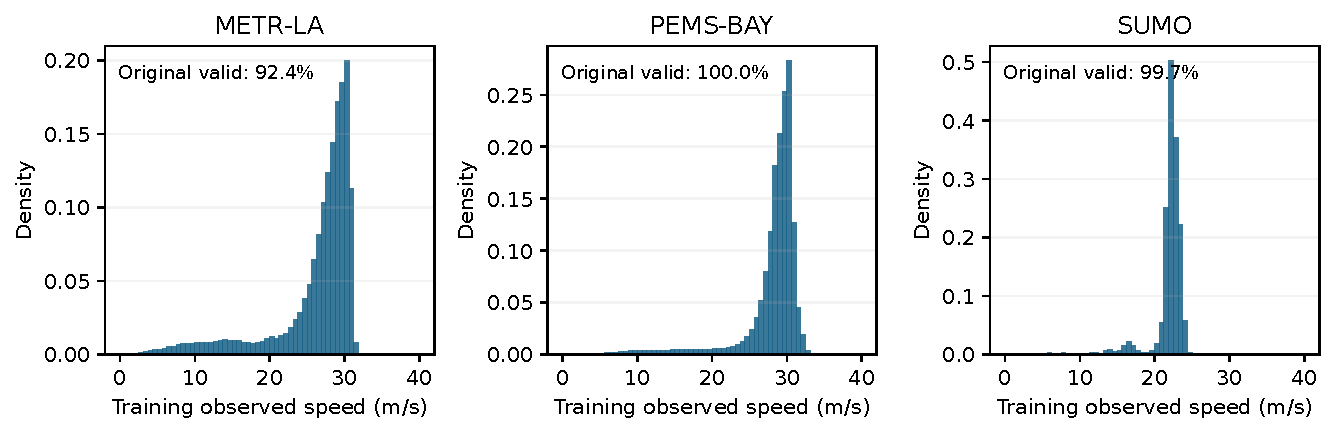
\includegraphics[width=\linewidth]{figures/data-profile.pdf}\caption{Training-partition observed-speed distributions before forecast-window construction. Only originally valid prepared measurements are plotted; labels report original valid fractions. SUMO includes its prepared training-partition measurements. The distributions are descriptive, not an explanation of calibration transfer.}\label{fig:data-profile}\end{figure}\clearpage
\begin{figure}[p]\centering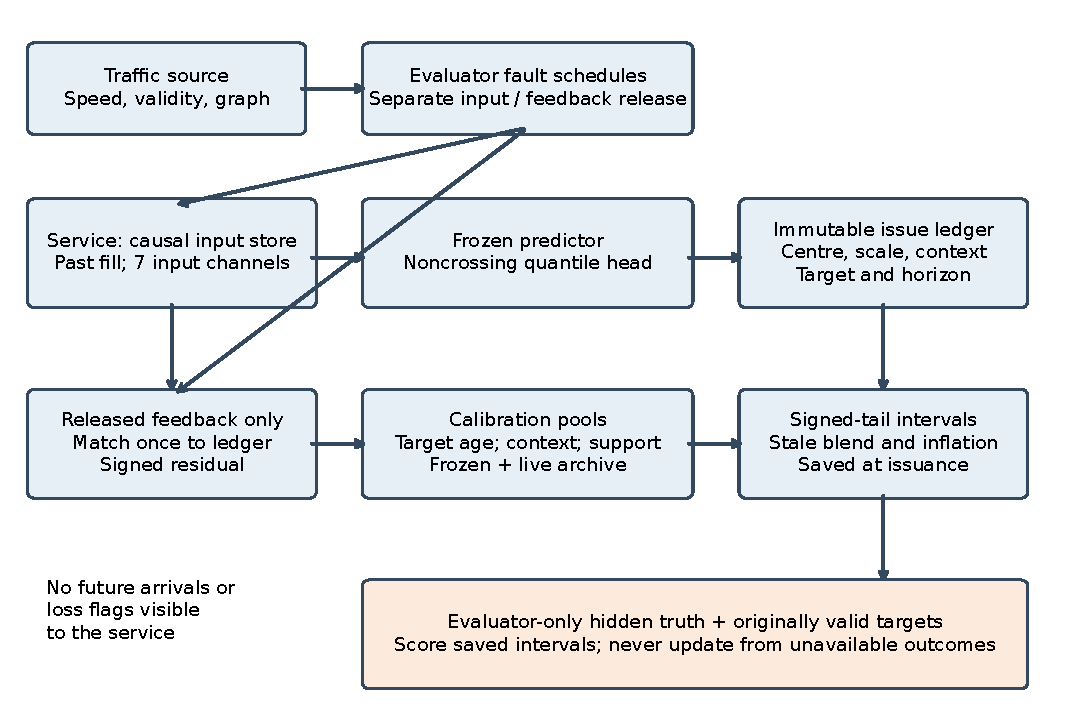
\includegraphics[width=\linewidth]{figures/architecture.pdf}\caption{Causal architecture with separate input, feedback and evaluator lanes. Stored issue records feed both residual matching and the calibration query; the junction is intentional. Hidden truth feeds scoring only. All module routes avoid text and preserve the service information boundary.}\label{fig:architecture}\end{figure}\clearpage
\begin{figure}[p]\centering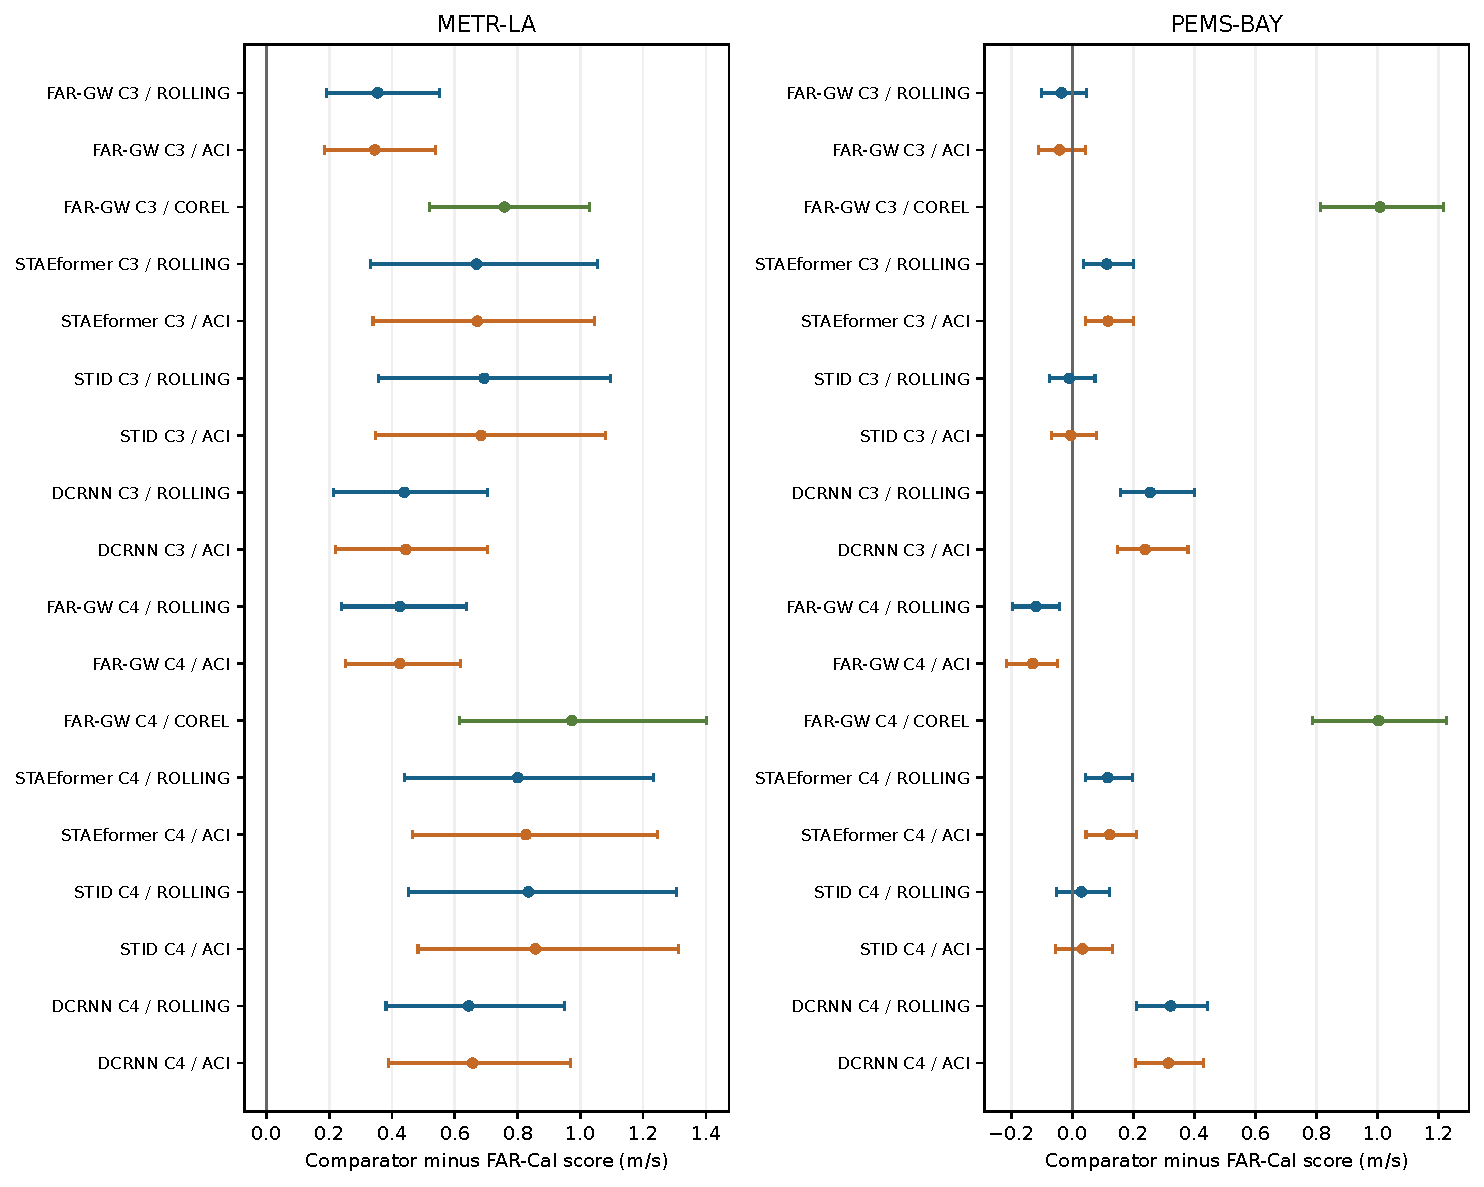
\includegraphics[width=\linewidth]{figures/benchmarks.pdf}\caption{Paired comparator-minus-FAR-Cal interval-score effects and 95\% intervals in SI units. Positive values favour FAR-Cal. Comparisons share frozen forecasts within each backbone; CoRel is restricted to FAR-GW.}\label{fig:benchmarks}\end{figure}\clearpage
\begin{figure}[p]\centering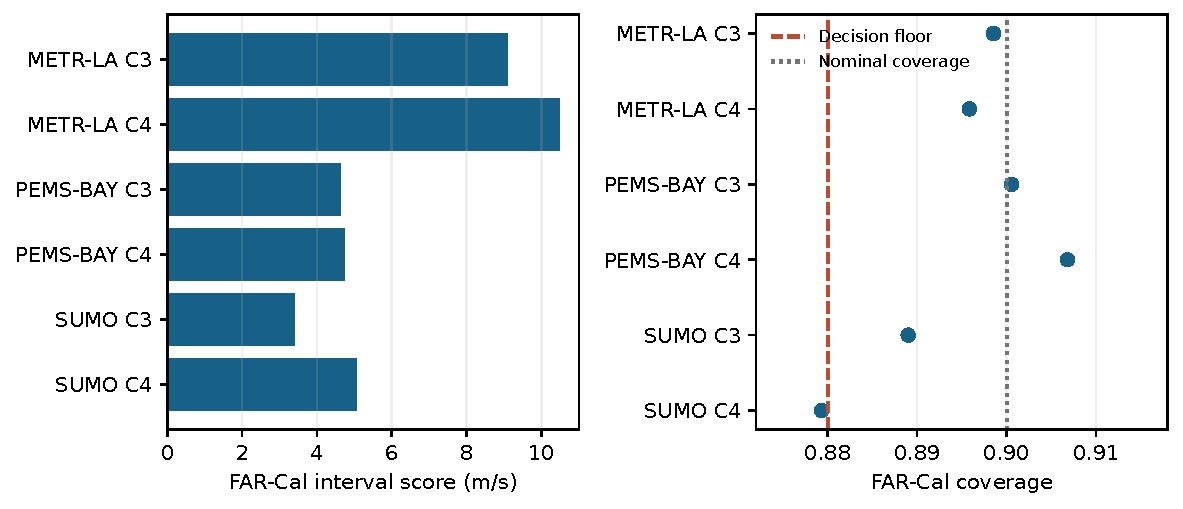
\includegraphics[width=\linewidth]{figures/quality.pdf}\caption{Final FAR-GW interval score and coverage for the six primary cells. Dashed and dotted lines mark the 0.88 decision floor and 0.90 nominal coverage. Absolute network scores are not a paired between-network effect.}\label{fig:quality}\end{figure}\clearpage
\begin{figure}[p]\centering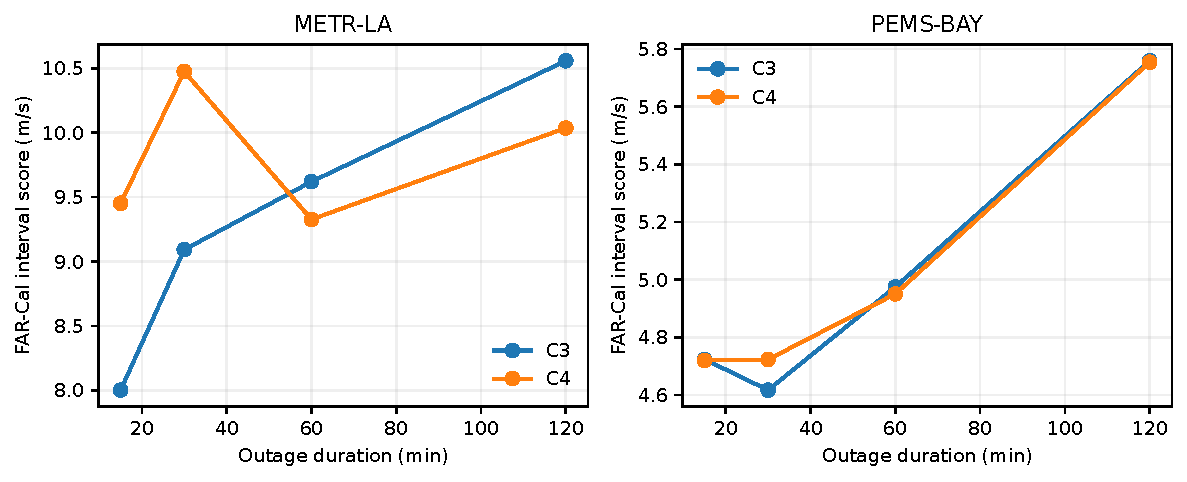
\includegraphics[width=\linewidth]{figures/duration.pdf}\caption{Interval score across the registered outage-duration grid. Lines connect descriptive scores, not interpolation guarantees; C3 and C4 are distinct feedback conditions.}\label{fig:duration}\end{figure}\clearpage
\begin{figure}[p]\centering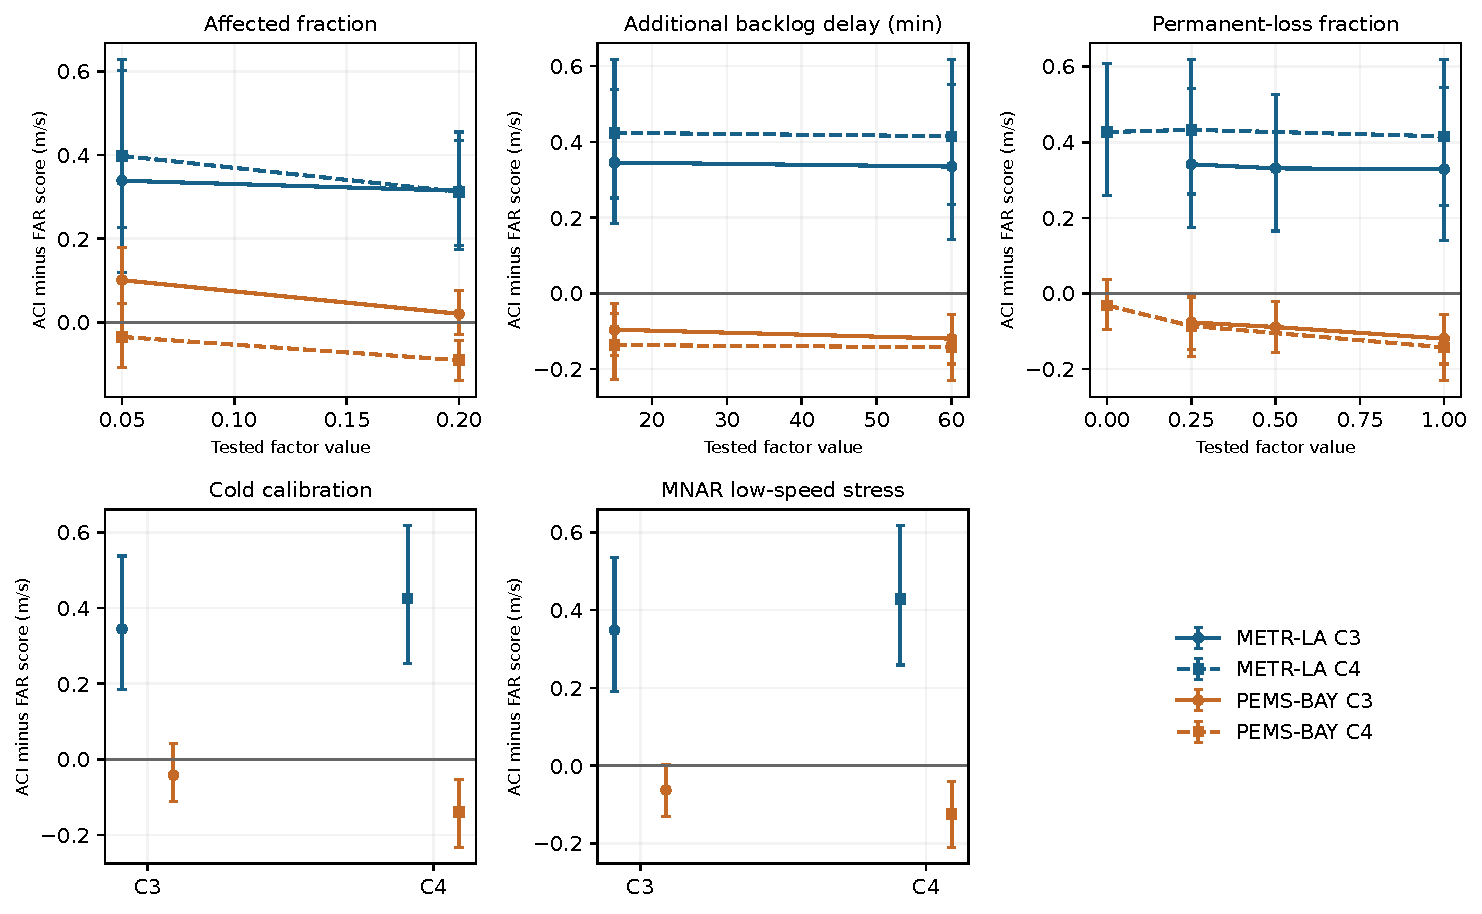
\includegraphics[width=\linewidth]{figures/stress.pdf}\caption{Additional one-factor stress: ACI-minus-FAR-Cal effects and paired 95\% intervals for affected fraction, backlog delay, permanent loss, cold calibration and MNAR. Positive values favour FAR-Cal. Categorical panels contain only their registered conditions; continuous lines connect tested values without extrapolation.}\label{fig:stress}\end{figure}\clearpage
\begin{figure}[p]\centering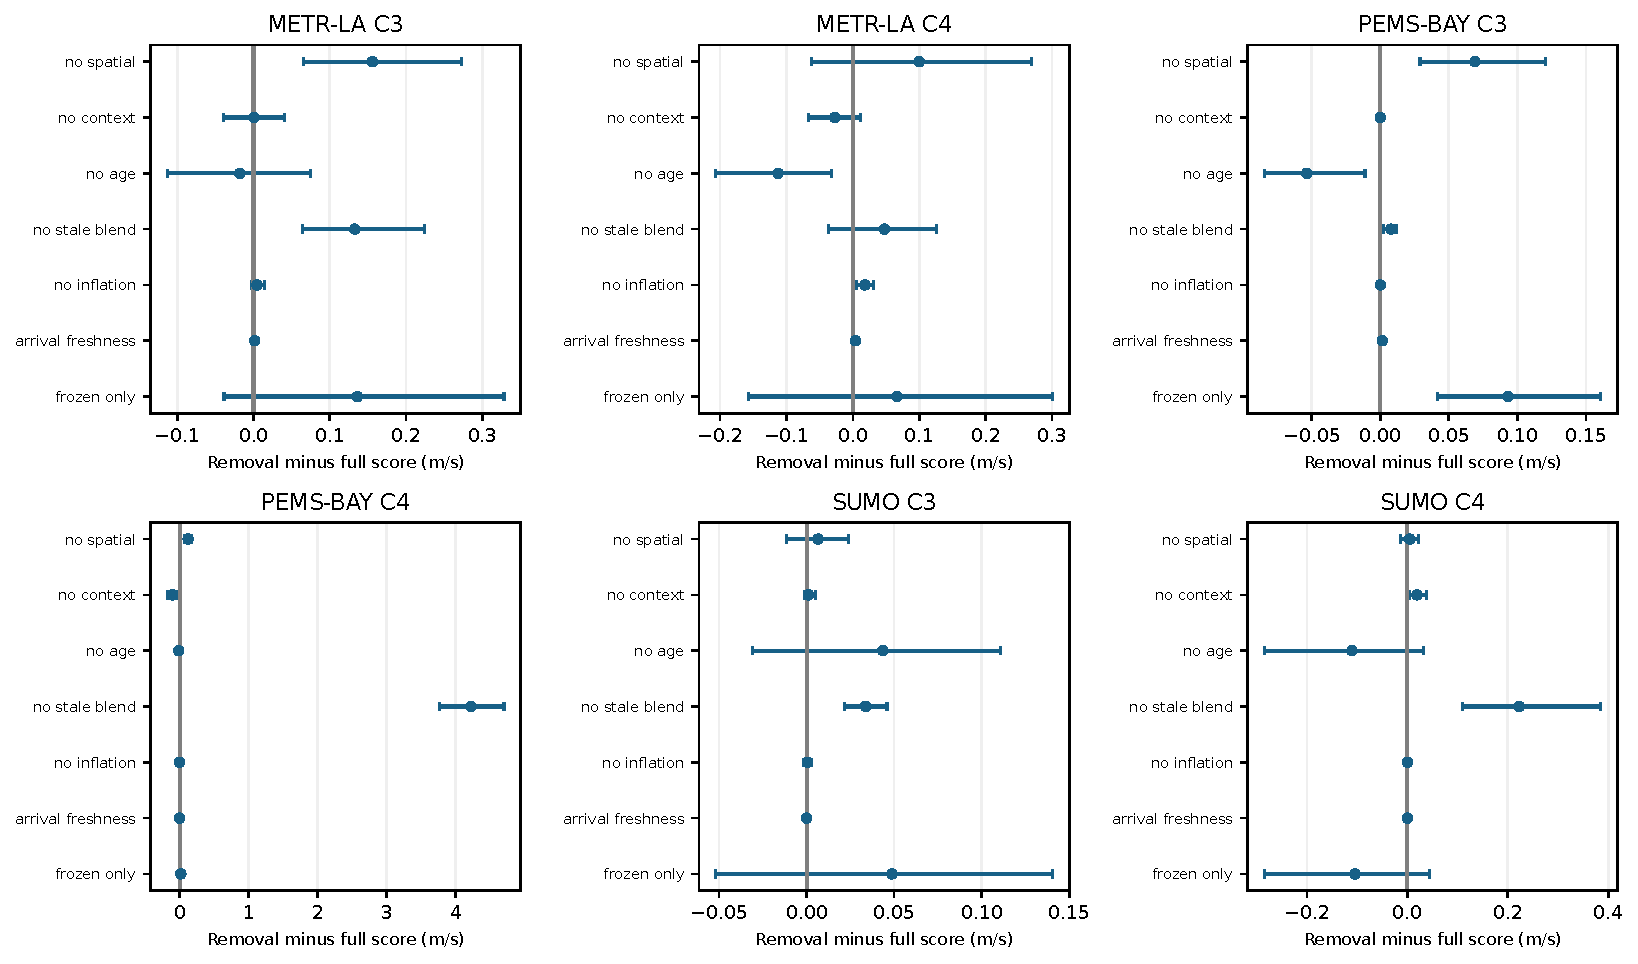
\includegraphics[width=\linewidth]{figures/ablations.pdf}\caption{Exploratory removal-minus-full interval-score effects and 95\% paired intervals. Positive values indicate deterioration after removal. Panel scales differ; the off-scale PEMS-BAY C4 stale-blend failure is explicitly labelled with its estimate and bounds.}\label{fig:ablations}\end{figure}\clearpage
\begin{figure}[p]\centering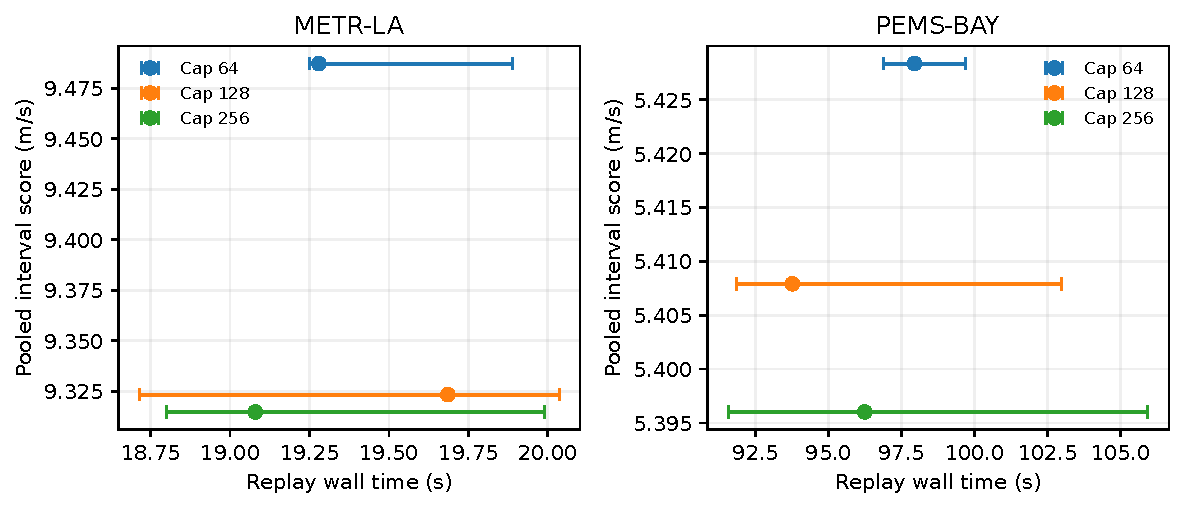
\includegraphics[width=\linewidth]{figures/compute.pdf}\caption{Descriptive archive-cap quality and wall-time sensitivity, with three observed runtime repetitions per cap and network. Horizontal bars are observed ranges, not confidence intervals. These fixed-run pooled scores differ from the origin-level paired inference estimand.}\label{fig:compute}\end{figure}\clearpage
\clearpage
\section*{Figure captions}
Figure 1. Training-partition observed-speed distributions before forecast-window construction. Only originally valid prepared measurements are plotted; labels report original valid fractions. SUMO includes its prepared training-partition measurements. The distributions are descriptive, not an explanation of calibration transfer.

Figure 2. Causal architecture with separate input, feedback and evaluator lanes. Stored issue records feed both residual matching and the calibration query; the junction is intentional. Hidden truth feeds scoring only. All module routes avoid text and preserve the service information boundary.

Figure 3. Paired comparator-minus-FAR-Cal interval-score effects and 95\% intervals in SI units. Positive values favour FAR-Cal. Comparisons share frozen forecasts within each backbone; CoRel is restricted to FAR-GW.

Figure 4. Final FAR-GW interval score and coverage for the six primary cells. Dashed and dotted lines mark the 0.88 decision floor and 0.90 nominal coverage. Absolute network scores are not a paired between-network effect.

Figure 5. Interval score across the registered outage-duration grid. Lines connect descriptive scores, not interpolation guarantees; C3 and C4 are distinct feedback conditions.

Figure 6. Additional one-factor stress: ACI-minus-FAR-Cal effects and paired 95\% intervals for affected fraction, backlog delay, permanent loss, cold calibration and MNAR. Positive values favour FAR-Cal. Categorical panels contain only their registered conditions; continuous lines connect tested values without extrapolation.

Figure 7. Exploratory removal-minus-full interval-score effects and 95\% paired intervals. Positive values indicate deterioration after removal. Panel scales differ; the off-scale PEMS-BAY C4 stale-blend failure is explicitly labelled with its estimate and bounds.

Figure 8. Descriptive archive-cap quality and wall-time sensitivity, with three observed runtime repetitions per cap and network. Horizontal bars are observed ranges, not confidence intervals. These fixed-run pooled scores differ from the origin-level paired inference estimand.
\end{document}
